\documentclass[11pt,a4paper]{article}
\usepackage[margin=1in]{geometry}
\usepackage[T1]{fontenc}
\usepackage{lmodern}
\usepackage{microtype}
\usepackage{amsmath,amssymb,mathtools}
\usepackage{enumitem}
\usepackage{xcolor}
\usepackage{amsthm}
\usepackage{hyperref}
\usepackage{float}
\usepackage{fancyhdr}
\usepackage{titlesec}
\usepackage{tikz-cd}
\usepackage{tikz}
\usetikzlibrary{arrows, matrix}
\usetikzlibrary{arrows.meta, angles, quotes, calc}
\usetikzlibrary{shapes, arrows, calc, arrows.meta, fit, positioning}%graphs,graphdrawing} %\usegdlibrary{layered}
\tikzset{
-Latex,auto,node distance =2 cm and 1.3 cm, thick,% node distance is the distance between one node to other, where 1.5cm is the length of the edge between the nodes  
state/.style ={circle, draw, minimum width = 0.9 cm}, % the minimum width is the width of the ellipse, which is the size of the shape of vertex in the node graph  
point/.style = {circle, draw, inner sep=0.18cm, fill, node contents={}},  
dotteddirected/.style={-Latex,loosely dash dot}, % it is the edge having two directions  
reverseedge/.style={-Latex,dotted}, % it is the dashed directed edge
el/.style = {inner sep=2.5pt, align=right, sloped}  
}
\hypersetup{colorlinks=true,linkcolor=blue!55!black,citecolor=blue!55!black,urlcolor=blue!55!black}
\setlength{\parskip}{5pt}
\setlength{\parindent}{0pt}
\setlist[enumerate]{leftmargin=*,itemsep=7pt}
\pagestyle{fancy}
\fancyhf{}
\lhead{\small Ph.D. Thesis Evaluation -- Response to Examiner}
\rhead{\small Avinash Kumar Dubey}
\cfoot{\thepage}

\usepackage{xparse}

% Automatic numbering of examiner comments
\newcounter{examcomment}

\renewcommand{\theexamcomment}{\arabic{examcomment}}
\newcommand{\comment}[1]{%
	\refstepcounter{examcomment}%
	\par\vspace{5pt}\noindent
	\colorbox{gray!13}{%
		\parbox{\dimexpr\linewidth-2\fboxsep}{%
			\textbf{Examiner's Comment \theexamcomment:} #1%
		}%
	}%
	\par
}

% Problem counter
\newcounter{problem}
\renewcommand{\theproblem}{\arabic{problem}}

% Problem environment: automatic or manually specified numbering
\NewDocumentEnvironment{problem}{o}
{%
	\par\vspace{5pt}\noindent
	\IfValueTF{#1}
	{\textbf{Problem #1.}}
	{%
		\refstepcounter{problem}%
		\textbf{Problem \theproblem.}%
	}%
	\quad\ignorespaces
}
{%
	\par\vspace{5pt}
}
%\newcommand{\comment}[1]{\vspace{5pt}\noindent\colorbox{gray!13}{\parbox{\dimexpr\linewidth-2\fboxsep}{\textbf{Examiner's comment:} #1}}}
\newcommand{\response}{\par\textbf{Response:} }
\newcommand{\revision}{\par\textbf{Proposed thesis revision:} }
\newcommand{\caution}[1]{\par\textit{\color{red!65!black}Action before submission: #1}}



\begin{document}

\begin{center}
{\Large\bfseries Consolidated Response to the Ph.D. Thesis Evaluation Reports}\\[6pt]
{\large\bfseries Responses to Prof. Debasish Ghose and Prof. Shubhendu Bhasin}\\[10pt]
\textbf{Candidate:} Avinash Kumar Dubey \qquad
\textbf{Roll No.:} 184076010\\
\textbf{Thesis:} \emph{Analysis \& Synthesis of Networked Dynamical Systems:
Stability, Performance and Applications of Consensus}
\end{center}
\vspace{4pt}
\hrule
\vspace{8pt}

This document consolidates the point-by-point responses to the evaluation
reports received from both examiners. Each examiner's comments and the
corresponding responses are presented in a separate section so that either
examiner can consult the complete set of comments and responses, including
those addressed to the other examiner. Chapter and section references refer
to the submitted thesis; page numbers will be updated after the revisions
are incorporated into the final thesis.

\section*{I. Responses to Prof. Debasish Ghose}
\textit{Department of Aerospace Engineering, Indian Institute of Science, Bengaluru}

Dear Professor Ghose,

I sincerely thank you for your positive evaluation of my thesis and for
recognizing its theoretical contributions and relevance to multi-agent
applications. I am grateful for the thoughtful questions and suggestions.
I respond to each point below and indicate the corresponding clarification
or revision proposed for the thesis.

\section*{Point-by-point responses}

\comment{The effect of a reverse edge in first-order and second-order system networks is well-known. Can it also be explained through the effect of feedback in LTI systems?}\label{DG:Feedback}
\response
Thank you for this insightful observation. Indeed, the effect of introducing a reverse edge in first-order and second-order consensus networks can also be interpreted through the classical feedback framework for linear time-invariant (LTI) systems. This interpretation provides an alternative control-theoretic explanation of the spectral changes induced by reverse edges and establishes a natural connection with the root-locus-based approach developed in Chapter~3.

Consider a directed path graph as the nominal network, with Laplacian matrix $\mathcal{L}_{\tau}$. The reverse edge from node $y$ to node $x$, where $y>x$, introduces a feedback connection based on the relative state between these two nodes (Refer Fig. \ref{fig:directed_path_reverse_edge}, $y=7$ and $x=3$ for the illustration). 


\begin{figure}[H]
	\centering
	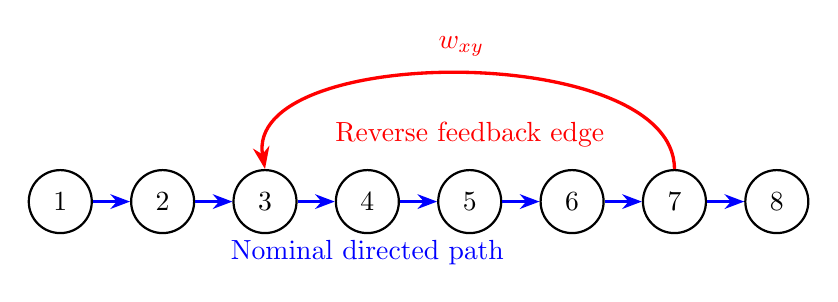
\begin{tikzpicture}[
		node distance=1.35cm,
		agent/.style={
			circle,
			draw,
			thick,
			minimum size=8mm,
			inner sep=0pt
		},
		nominal/.style={
			-{Stealth[length=2.5mm]},
			thick,
			blue
		},
		feedback/.style={
			-{Stealth[length=2.8mm]},
			very thick,
			red
		}
		]
		
		% Nodes
		\foreach \i in {1,...,8}
		\node[agent] (v\i) at (1.3*\i,0) {$\i$};
		
		% Nominal directed path
		\foreach \i [evaluate=\i as \j using int(\i+1)] in {1,...,7}
		\draw[nominal] (v\i) -- (v\j);
		
		% Reverse edge from y to x
		\draw[feedback]
		(v7.north) to[out=90,in=100,looseness=0.8]
		node[midway,above=0.8mm,red] {$w_{xy}$}
		(v3.north);
		
		% Labels
		\node[blue] at (5.2,-0.65)
		{Nominal directed path};
		
		\node[red] at (6.5,0.85)
		{Reverse feedback edge};
		
	\end{tikzpicture}
	\caption{Directed path graph with a reverse edge from node $y$ to node $x$, where $y>x$.}
	\label{fig:directed_path_reverse_edge}
\end{figure}


Let
\[
b=e_x,\qquad c=e_x-e_y,
\]
where $e_i$ denotes the $i$th standard basis vector. The reverse edge measures the relative state $c^T\boldsymbol{x}=x_x-x_y$ and feeds the resulting signal back to node $x$ with weight $w_r>0$. The corresponding feedback input is
\[
u_r=-w_r c^T\boldsymbol{x},
\]
which is injected through $b$.

\textit{First-order consensus:}
For the nominal path network, the first-order consensus dynamics are
\[
\boldsymbol{\dot{x}}=-\mathcal{L}_{\tau}\boldsymbol{x}.
\]
After introducing the reverse edge, the dynamics become
\begin{equation}
\boldsymbol{\dot{x}}
=-\mathcal{L}_{\tau}\boldsymbol{x}-bw_rc^T\boldsymbol{x}
=-\left(\mathcal{L}_{\tau}+w_rbc^T\right)\boldsymbol{x}.
\label{eq:reverse_edge_first_order}
\end{equation}
Thus, the reverse edge can be interpreted as a constant-gain feedback connection around the nominal path network. The corresponding transfer function from the scalar feedback input to the relative-state output is
\begin{equation}
G_{\tau}(s)=c^T(sI+\mathcal{L}_{\tau})^{-1}b.
\end{equation}
Using the matrix determinant lemma \cite{harville1997}, the closed-loop characteristic equation associated with the disagreement dynamics takes the classical feedback form
\begin{equation}
1+w_rG_{\tau}(s)=0.
\label{eq:reverse_edge_feedback_first_order}
\end{equation}
Since $c^T\mathbf{1}=0$, the feedback does not affect the consensus mode corresponding to the zero Laplacian eigenvalue. Its effect is therefore confined to the disagreement dynamics.

In the first-order network, the nonzero Laplacian eigenvalues determine the decay rates of the disagreement modes. Introducing a reverse edge modifies these eigenvalues and consequently changes the convergence rate. In the chain configurations investigated in the thesis, the dominant disagreement eigenvalue moves closer to the origin, reducing the asymptotic convergence rate while preserving consensus stability under the directed spanning-tree condition.

\textit{Second-order consensus:}
The same feedback interpretation extends to the double-integrator network. The nominal dynamics are
\begin{equation}
\dot{\bf{x}}=\bf{v},\qquad
\dot{\bf{x}}=-\mathcal{L}_{\tau}\bf{x}-\gamma \mathcal{L}_{\tau}\bf{v},
\end{equation}
where $\gamma$ denotes the velocity coupling gain. Under the second-order consensus protocol, the reverse edge introduces the feedback signal
\[
u_r=-w_r(c^T\bf{x}+\gamma c^T \bf{v}),
\]
which is injected into the acceleration equation through $b$. The resulting closed-loop dynamics are
\begin{equation}
\begin{aligned}
\dot{\bf{x}}&=\bf{v},\\
\dot{\bf{v}}&=-\mathcal{L}_{\tau}\bf{x}-\gamma \mathcal{L}_{\tau}\bf{v}
- bw_rc^T(x+\gamma \bf{v}).
\end{aligned}
\label{eq:reverse_edge_second_order}
\end{equation}

The corresponding nominal transfer function from the scalar acceleration input to the relative-state feedback output is
\begin{equation}
G_{\tau}(s)
=(1+\gamma s)c^T
\left(s^2I+\gamma s\mathcal{L}_{\tau}+\mathcal{L}_{\tau}\right)^{-1}b.
\label{eq:second_order_feedback_tf}
\end{equation}
Consequently, the reverse-edge feedback gives the closed-loop characteristic equation
\begin{equation}
1+w_rG_{\tau}(s)=0,
\label{eq:reverse_edge_feedback_second_order}
\end{equation}
when considered on the disagreement dynamics.

The difference between first-order and second-order networks becomes particularly important when examining the closed-loop poles. For a nonzero Laplacian eigenvalue $\lambda$, the corresponding second-order characteristic equation is
\begin{equation}
s^2+\gamma\lambda s+\lambda=0.
\end{equation}
For a directed network, the Laplacian eigenvalues need not be real. Thus, introducing reverse edges can modify both the real and imaginary parts of the Laplacian spectrum, thereby changing the damping and oscillatory characteristics of the second-order modes. In particular, the complex nature of the affected eigenvalues can reduce the stability margin, and if the velocity coupling gain is insufficient, the corresponding closed-loop poles may enter the right-half plane, resulting in loss of consensus.

Therefore, while the effect of a reverse edge in a first-order network is primarily reflected in a change in the disagreement decay rates, its effect in a second-order network can be more critical because it may also affect closed-loop stability.

\textit{Connection with directed incidence matrices and feedback design:}
This feedback interpretation can also be expressed through an incidence-matrix factorization of the directed Laplacian. Let $E$ denote the node-edge incidence matrix, whose column for a directed edge $j\rightarrow i$ is $e_i-e_j$. Let $E_{\mathrm{in}}$ denote the corresponding receiving-node incidence matrix, whose column for the same edge is $e_i$, and let $W$ be the diagonal matrix of edge weights. With this convention, the directed Laplacian admits the asymmetric factorization
\begin{equation}
\mathcal{L}=E_{\mathrm{in}}WE^T.
\label{eq:directed_laplacian_factorization}
\end{equation}
This factorization separates the relative-state measurement across an edge from the node at which the corresponding feedback signal is injected. In this sense, each directed edge represents a localized feedback connection within the overall network.

Finally, this viewpoint provides a natural control-theoretic interpretation of the root-locus-based method developed

\comment{In Chapter 2, can Cases 5 and 6 be considered special cases of Case 4? Or do they have to be treated separately?}
\response
The relationship between Cases 4, 5, and 6 can be clarified by examining their characteristic equations and the corresponding changes in the in-degree structure of the network.

\textbf{Case 4 Fully Nested Cycles with Disjoint Reverse Edges}

The case 4 is shown in Figure \ref{Case4}.


 \begin{figure}[H]
		\centering
		\scalebox{0.7}{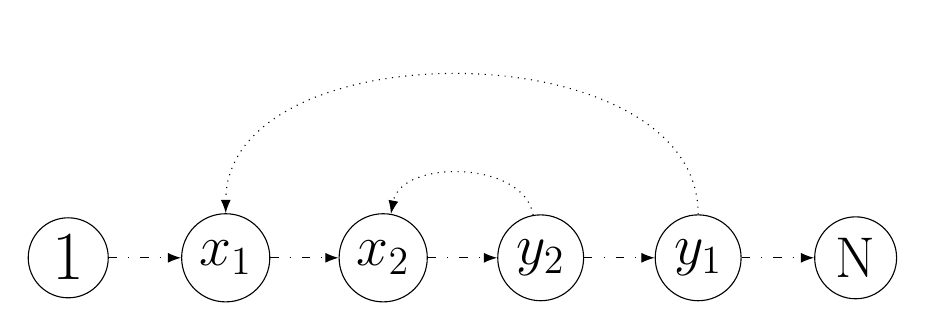
\begin{tikzpicture}
				\node[state] (root) {\Huge{$1$}};
				\node[state] (x1) [right of=root] {\huge{$x_1$}};
				\node[state] (x2) [right of=x1] {\huge{$x_2$}};
				\node[state] (y2) [right of=x2] {\huge{$y_2$}};
				\node[state] (y1) [right of=y2] {\huge{$y_1$}};
				\node[state] (N) [right of=y1] {\huge{N}};
				\path [dotteddirected] (root) edge (x1);
				\path [dotteddirected] (x1) edge (x2);
				\path [dotteddirected] (x2) edge (y2);
				\path [dotteddirected] (y2) edge (y1);
				\path [dotteddirected] (y1) edge (N);
				\path[reverseedge] (y1) edge[bend right=90] (x1);
				\path[reverseedge] (y2) edge[bend right=80] (x2);
		\end{tikzpicture}}
		\caption{Fully overlapping but reverse edges do not share nodes}
		\label{Case4}
	\end{figure} 
\medskip
\noindent

In Case 4, Cycle 2 is strictly contained within Cycle 1. Hence, the two reverse edges don't share either the head node or the tail node with each other i.e.,
\begin{equation}
    x_1 < x_2 < y_2 < y_1,
    \qquad \ell_1 > \ell_2.
\end{equation}
The  characteristics equation obtained for Case 4 in 2.57 is :
\begin{equation}\label{eq:case4_theorem_statement}
	s^{\ell_1+1} + 2s^{\ell_1} + s^{\ell_1-1} - s^{\ell_1-\ell_2} - s^{\ell_1-\ell_2-1} = 1.
\tag{2.57}
\end{equation}
\textbf{Case 5: Fully nested cycles sharing a common tail}

The case 5 is shown in Figure \ref{Case5}.
\begin{figure}[H]
		\centering
		\scalebox{0.55}{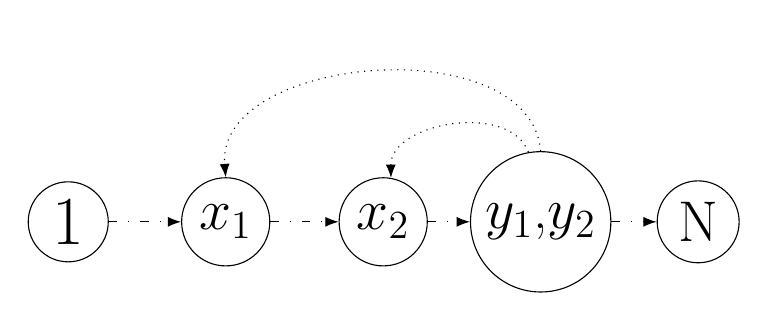
\begin{tikzpicture}
				\node[state] (root) {\Huge{$1$}};
				\node[state] (x1) [right of=root] {\huge{$x_1$}};
				\node[state] (x2) [right of=x1] {\huge{$x_2$}};
				\node[state] (y1) [right of=x2] {\huge{$y_1$,$y_2$}};
				\node[state] (N) [right of=y1] {\huge{N}};
				\path [dotteddirected] (root) edge (x1);
				\path [dotteddirected] (x1) edge (x2);
				\path [dotteddirected] (x2) edge (y1);
				\path [dotteddirected] (y1) edge (N);
				\path[reverseedge] (y1) edge[bend right=90] (x1);
				\path[reverseedge] (y1) edge[bend right=80] (x2);
		\end{tikzpicture}}
		\caption{Fully overlapping with shared tail node between the two reverse edges}
		\label{Case5}
	\end{figure}


In Case 5, the two reverse edges share a common tail node, i.e.,
\begin{equation}
    x_1 < x_2 < y_1 = y_2,
    \qquad \ell_1 > \ell_2.
\end{equation}

Although the two reverse edges originate from the same node, they terminate at two distinct head nodes, $x_1$ and $x_2$. Consequently, the additional incoming-edge contributions are distributed across two different rows of the in-degree Laplacian. In particular, both head nodes receive one additional incoming edge, while the common tail node does not receive any additional incoming edge from these reverse edges.

The characteristic equation obtained for Case 5 in (2.60) is
\begin{equation}
    (s+1)^2s^{\ell_1-1}
    -(s+1)s^{\ell_1-\ell_2-1}-1=0.
    \tag{2.60}
\end{equation}

Expanding the above expression gives
\begin{equation}
\begin{aligned}
    s^{\ell_1+1}
    +2s^{\ell_1}
    +s^{\ell_1-1}
    -s^{\ell_1-\ell_2}
    -s^{\ell_1-\ell_2-1}
    =1.
\end{aligned}
\tag{2.60a}
\end{equation}

This is exactly the characteristic equation obtained for Case 4 in (2.57).
%\begin{equation}
%\begin{aligned}
%    s^{\ell_1+1}
%    +2s^{\ell_1}
%    +s^{\ell_1-1}
%    -s^{\ell_1-\ell_2}
%    -s^{\ell_1-\ell_2-1}
%    =1.
%\end{aligned}
%\tag{2.57}
%\end{equation}

Therefore, \textbf{Case 5 can be considered a special case of Case 4 from the perspective of the characteristic equation and the resulting spectral stability boundary}. A separate spectral derivation is not necessary for the in-degree Laplacian formulation considered in this thesis.

\medskip
\noindent
\textbf{Case 6: Fully nested cycles sharing a common head}

The case 6 is shown in Figure \ref{Case6}.

\begin{figure}[H]
		\centering
		\scalebox{0.55}{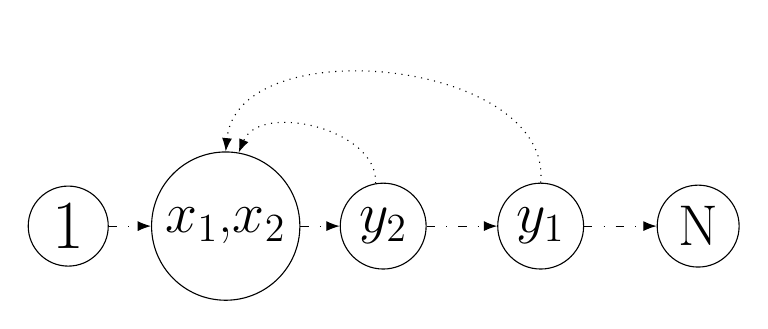
\begin{tikzpicture}
				\node[state] (root) {\Huge{$1$}};
				\node[state] (x1) [right of=root] {\huge{$x_1$,$x_2$}};
				\node[state] (y2) [right of=x1] {\huge{$y_2$}};
				\node[state] (y1) [right of=y2] {\huge{$y_1$}};
				\node[state] (N) [right of=y1] {\huge{N}};
				\path [dotteddirected] (root) edge (x1);
				\path [dotteddirected] (x1) edge (y2);
				\path [dotteddirected] (y2) edge (y1);
				\path [dotteddirected] (y1) edge (N);
				\path[reverseedge] (y1) edge[bend right=90] (x1);
				\path[reverseedge] (y2) edge[bend right=80] (x1);
		\end{tikzpicture}}
		\caption{Fully overlapping with shared head node between the two reverse edges}
		\label{Case6}
	\end{figure}

In Case 6, the two reverse edges share a common head node, i.e.,
\begin{equation}
    x_1 = x_2 < y_2 < y_1,
    \qquad \ell_1 > \ell_2.
\end{equation}

Unlike Case 5, both reverse edges terminate at the same node. Thus, the common head node receives two additional incoming edges. Since it also receives the original incoming edge from its predecessor along the directed chain, its in-degree becomes three:
\begin{equation}
    d_{\mathrm{in},x_1}=3.
\end{equation}

This changes the corresponding diagonal entry of the in-degree Laplacian and, consequently, the characteristic equation. The determinant obtained for Case 6 in (2.62) is
\begin{equation}
\begin{aligned}
    |\lambda I-L|
    ={}&\lambda(\lambda-1)^{N-\ell_1-1}\\
    &\times\left[
    (\lambda-1)^{\ell_1}(\lambda-2)
    +(\lambda-1)^{\ell_1-\ell_2}-1
    \right]=0.
\end{aligned}
\tag{2.62}
\end{equation}

Using the substitution $s=1-\lambda$, the corresponding characteristic equation becomes
\begin{equation}
    s^{\ell_1}(s+2)-s^{\ell_1-\ell_2}=1.
    \tag{2.61}
\end{equation}

This is different from the characteristic equation obtained for Case 4. Hence, \textbf{Case 6 cannot be treated as a special case of Case 4 under the in-degree Laplacian formulation considered in this thesis and requires a separate spectral analysis.}

\medskip
\noindent
\textbf{Additional clarification on the incidence representation}

The distinction also highlights the role of the chosen Laplacian formulation. The present thesis employs the in-degree Laplacian,
\begin{equation}
    L=D_{\mathrm{in}}-W_g,
\end{equation}
for which the receiving (head) nodes determine the rows in which the additional reverse-edge contributions appear. Under an out-degree Laplacian formulation, the corresponding structural effect would instead be associated with the sending (tail) nodes. For example, two reverse edges sharing a common tail would contribute to the out-degree of the same node. Thus, the spectral equivalence observed between Cases 4 and 5 is specific to the in-degree Laplacian formulation adopted here and should not be interpreted as a topology-independent equivalence.

\medskip
\noindent
\textbf{In summary}, Cases 4, 5, and 6 represent three distinct topological configurations. However, for the in-degree Laplacian studied in this thesis, Case 5 yields the same characteristic equation as Case 4, whereas Case 6 produces a distinct characteristic equation due to the accumulation of incoming edges at the common head node. Accordingly, Case 5 is spectrally reducible to Case 4, while Case 6 requires separate treatment.

\comment{I am a little confused about Fig. 3.5. The disc around $p_{\ell+1}$ should have a radius $p_1$. I am not sure if this is the case in the figure. Maybe it is an issue of scale?}
\response
Thank you for pointing this out. The original Figure 3.5 was not drawn to the correct scale, which made the radius of the disc corresponding to $p_{\ell+1}$ appear inconsistent. As correctly noted, this disc should have a radius of $p_1$. 

In the column Gershgorin construction associated with $\widetilde P$, based on Gershgorin's disc theorem \cite{horn2012matrix}, the last column disc is centered at $p_{\ell+1}$ and has radius $p_1$, as stated immediately before (3.18). Its leftmost real-axis point is therefore $p_{\ell+1}-p_1$. For the numerical illustration in Figure 3.5, $p_1=12$, $\ell=5$, and the arithmetic-progression spacing is $d=2$. The last disc is consequently centered at $p_{\ell+1}=2p_1-\ell d=14$ and has radius $12$, so its left boundary is at $14-12=2=d$. The geometry is consistent with the analytical construction; the figure's scale/labels may not make the radius sufficiently apparent. I have altered Figure 3.5 to accurately reflect the prescribed disc radii and their geometric relationships.
Figure 3.5 is reproduced here as Figure~\ref{fig:GersgorinDiscInAP}.
\begin{figure}[H]
	\centering
	\resizebox{0.75\textwidth}{!}{%
	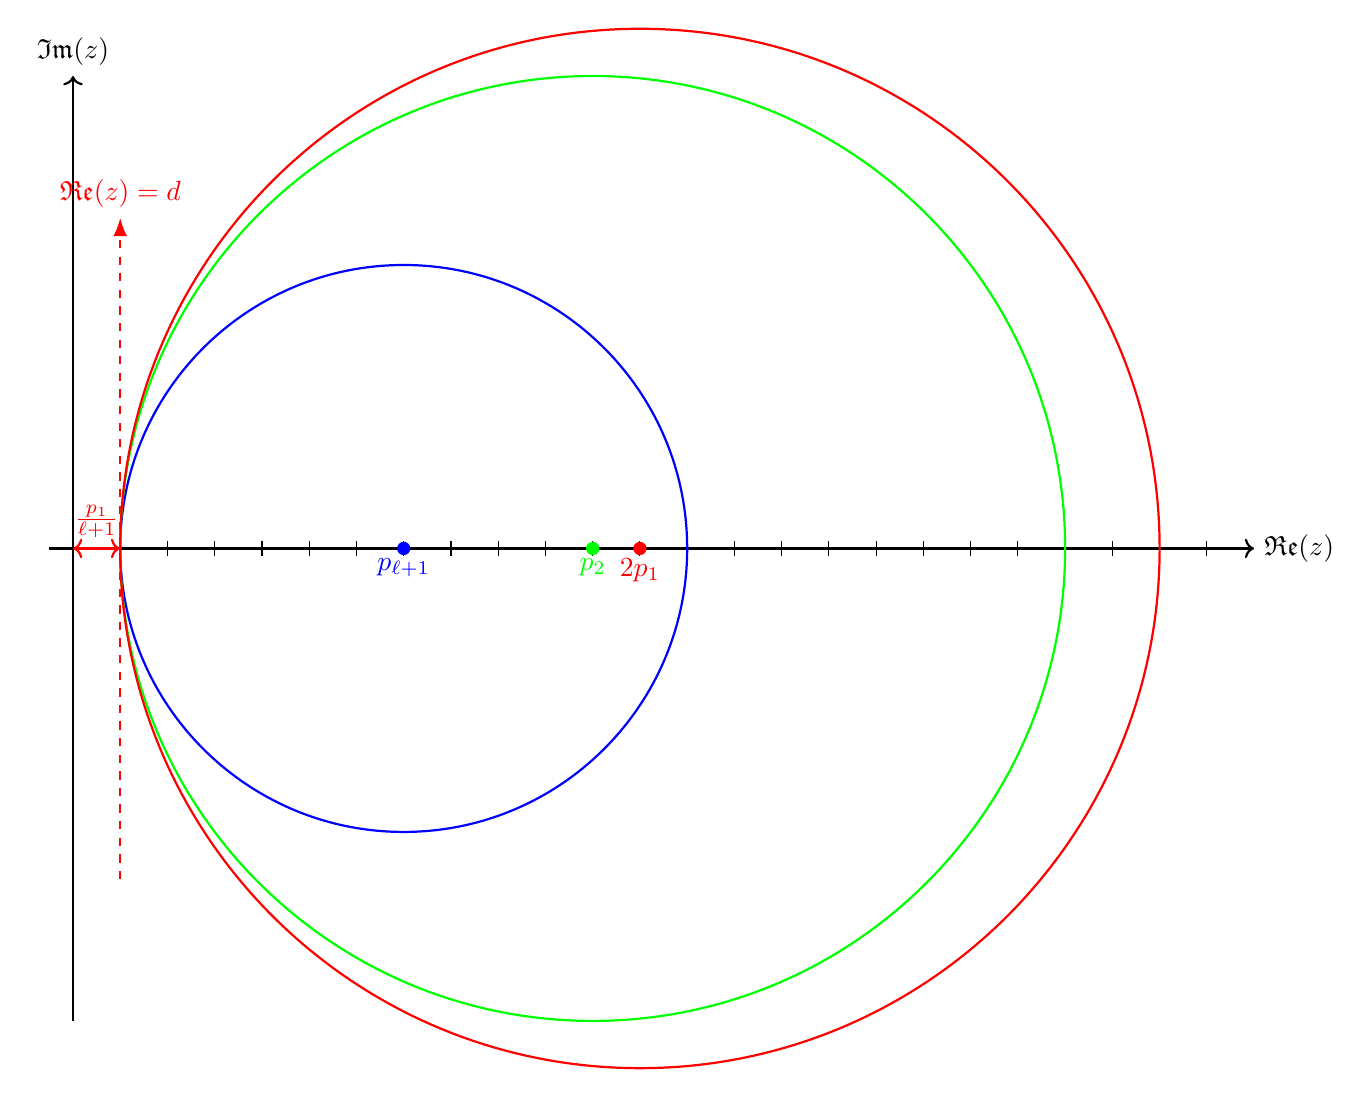
\begin{tikzpicture}[scale=0.3]
		\draw[->, thick] (-1,0) -- (50,0) node[right] {$\mathfrak{Re}(z)$};
		\draw[->, thick] (0,-20) -- (0,20) node[above] {$\mathfrak{Im}(z)$};
        \foreach \x in {2, 4, 6, 8, 10, 12, 14, 16, 18, 20, 22, 24, 26, 28, 30, 32, 34, 36, 38, 40, 42, 44, 46, 48}
		\draw[-] (\x, -0.3) -- (\x, 0.3);
		\draw[dashed, red, thick] (2,-14) -- (2,14) node[above] {$\mathfrak{Re}(z) = d$};
		
		\draw[draw=blue, thick] (14.0,0) circle (12cm);
		\fill[blue] (14.0,0) circle (8pt) node[below] {$p_{\ell+1}$};
		
		\draw[draw=green, thick] (22,0) circle (20.0cm);
		\fill[green] (22,0) circle (8pt) node[below] {$p_2$};
		
		\draw[draw=red, thick] (24.0,0) circle (22cm);
		\fill[red] (24.0,0) circle (8pt) node[below] {$2p_1$};
		
		\draw[<->, thick, red] (0,0) -- (2,0) node[midway, above] {$\frac{p_1}{\ell+1}$};
	\end{tikzpicture}
}
	\caption{Gershgorin column discs for $\tilde{P}$ when scaling parameters $p_i$ form an optimal Arithmetic Progression ($p_1 = 12, \ell = 5, d = 2$). All discs touch the boundary line $\mathfrak{Re}(z) = d$.}
	\label{fig:GersgorinDiscInAP}
\end{figure}


\comment{Given the constraints set out in Problem 5.3, I would expect feasibility, or existence of solution, based on initial conditions, to be an issue. I wonder if these were explicitly established based on the constraints, taken together or individually.}

\response

Thank you for raising this important point. I agree that the feasibility of Problem 5.3(reproduced below with corresponding engagement geometry in Fig. \ref{fig:ch_DP_eng_geometry}) should be understood in terms of the simultaneous satisfaction of all four requirements: target interception, terminal impact-angle satisfaction, prescribed impact time, and actuator feasibility. 
\begin{problem}[5.3]\label{prob:ch_DP_main_problem}
	Given an interceptor's initial state vector $\mathbf{x}(0) = [x_M(0), y_M(0), \gamma_M(0)]^T = [0, 0, \gamma_M(0)]^T$, constant speed $V_M$, target initial location $(r_0, 0)$, and maximum lateral acceleration capability $a^{\max}$, synthesize a computationally efficient, singularity-free guidance law $a_M(t)$ such that the following conditions are met:
	\begin{enumerate}
		\item \textbf{Target Interception:} The interceptor reaches the target position at time $t = t_{\text{imp}}$, satisfying $r(t_{\text{imp}}) = 0$.
		\item \textbf{Impact Angle Satisfaction:} The velocity vector aligns with the desired approach angle at interception: $\gamma_M(t_{\text{imp}}) = \theta_t$.
		\item \textbf{Impact Time Satisfaction:} Interception occurs exactly at a designated feasible arrival time $t_{\text{imp}} = t^{\star}$.
		\item \textbf{Actuator Feasibility:} The lateral acceleration input satisfies the strict bound $|a_M(t)| \le a^{\max}$ for all $t \in [0, t^{\star}]$.
	\end{enumerate}
\end{problem}


\begin{figure}[H]
	\centering
	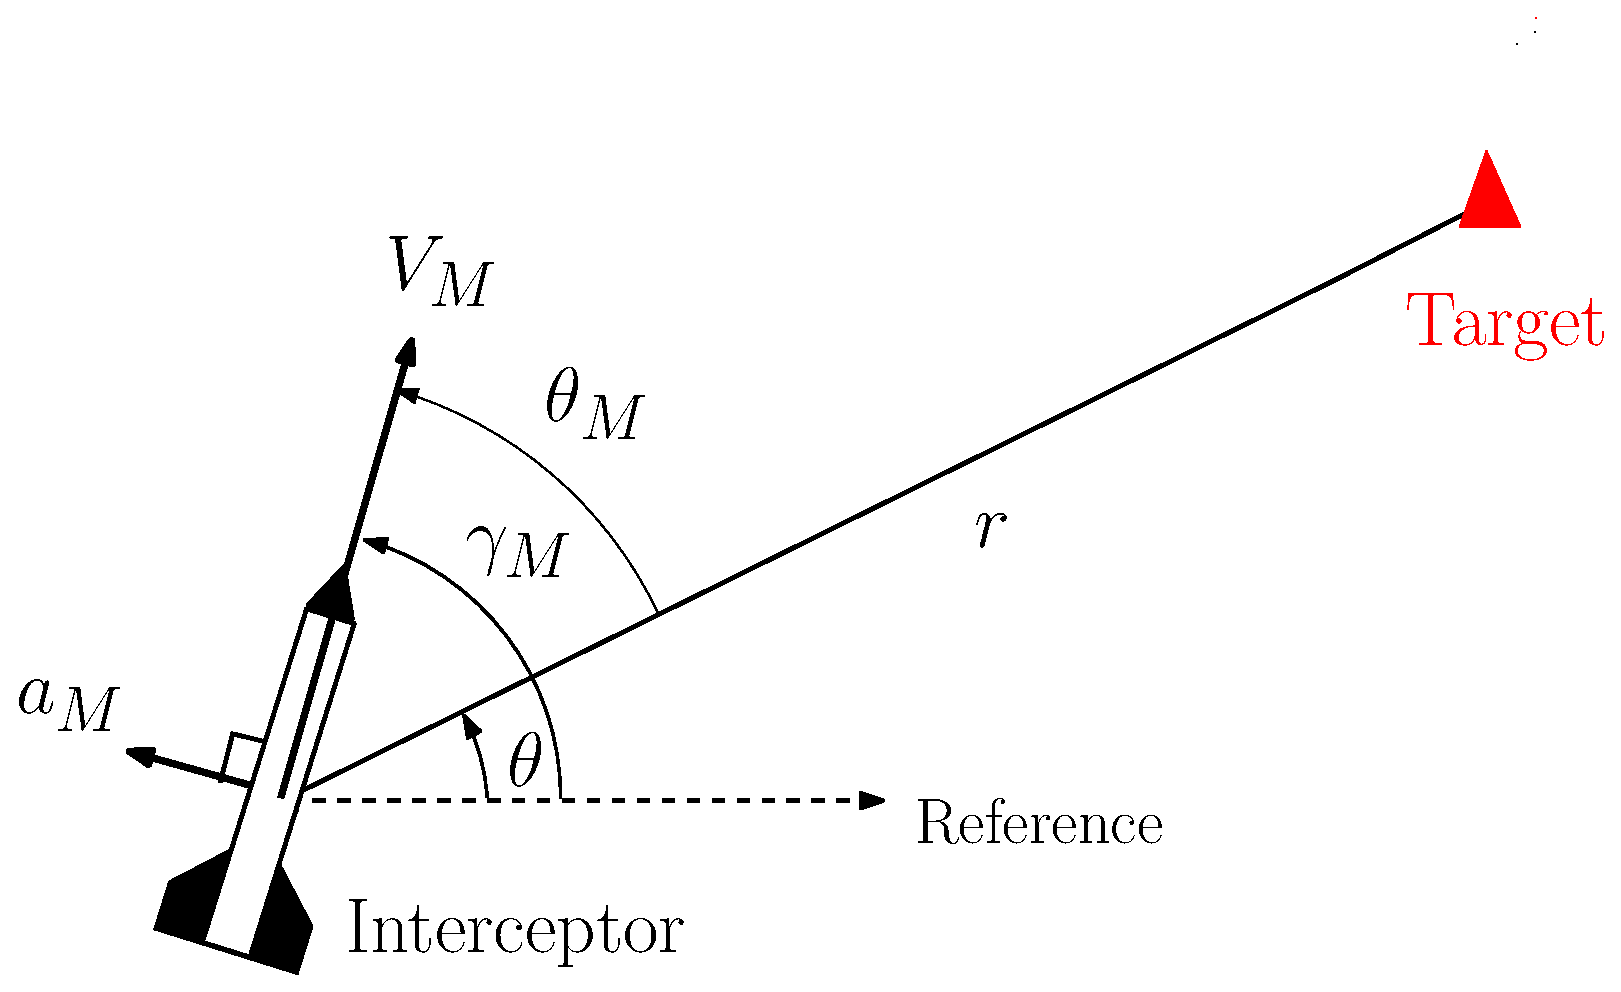
\includegraphics[width=0.8\textwidth, keepaspectratio]{5_Images/dubins_eng.eps}
	\caption{Planar engagement geometry between an autonomous interceptor and a stationary target.}
	\label{fig:ch_DP_eng_geometry}
\end{figure}


These requirements are not independently feasible for arbitrary initial conditions and arbitrary prescribed impact times. The existence of a solution is established through the geometric trajectory constructions developed in Sections 5.3.3--5.3.6.

For a given initial configuration and desired terminal impact angle, the classical Dubins path provides the minimum feasible path length $P_{\min}$ and, consequently, the minimum achievable impact time:
\[
t_{\mathrm{imp}}^{\min}=\frac{P_{\min}}{V_M}.
\]
Therefore, a necessary condition for feasibility is
\[
t^\star_{\mathrm{imp}}\geq t_{\mathrm{imp}}^{\min}.
\]

The actuator constraint determines the minimum permissible turning radius:
\[
r_m=\frac{V_M^2}{a_{\max}}.
\]
The proposed Dubins-like construction uses this radius for the primary circular arc, a straight-line tangent segment, and a secondary circular arc with a design radius $r_d\geq r_m$. Thus, the lateral acceleration on the secondary arc satisfies
\[
|a_M|=\frac{V_M^2}{r_d}
\leq \frac{V_M^2}{r_m}=a_{\max},
\]
while the straight segment requires zero lateral acceleration. Hence, the actuator constraint is respected by construction.

Regarding geometric feasibility, Section 5.3.3 derives the standard Transverse Common Tangent (TCT) construction and its corresponding geometric conditions. In particular, the circles must admit a valid common tangent, requiring
\[
d(r_d)\geq r_m+r_d.
\]
For the same-sign angle configuration considered in this section, this condition imposes the design interval
\[
r_d\in[r_m,r_{\mathrm{crit}}^{\mathrm{TCT}}).
\]
The resulting path length $P(r_d)$, and hence the impact time $t_{\mathrm{imp}}(r_d)=P(r_d)/V_M$, can be continuously tuned over the attainable interval. Section 5.3.6 further establishes the path-length monotonicity underlying this time-tuning mechanism. Consequently, a prescribed impact time within this interval can be achieved by selecting a suitable secondary radius.

The standard TCT construction, however, imposes an upper bound on the achievable arrival time. To overcome this limitation, Section 5.3.4 introduces the mirrored TCT geometry. In this configuration, the center-to-center distance increases monotonically with the mirrored secondary radius, and the resulting path length is unbounded above. The analysis therefore establishes that any physically feasible prescribed impact time satisfying
\[
t^\star_{\mathrm{imp}}\geq t_{\mathrm{imp}}^{\min}
\]
can be matched by selecting a suitable mirrored-circle radius $r'_d$. The additional DCT and outer-circle configurations are also discussed in Section 5.3.5 for the corresponding geometric cases.

Thus, the existence of a solution is conditional on the joint geometric and actuator feasibility conditions of the selected path construction. The minimum Dubins path establishes the lower bound on achievable impact time, while the variable-radius and mirrored geometries provide the required flexibility to achieve the prescribed arrival time without violating the acceleration constraint. The thesis therefore does not claim feasibility for arbitrary combinations of initial conditions, terminal impact angles, and arrival times.

We acknowledge that these feasibility conditions can be stated more explicitly in the formal problem formulation. Accordingly, we will strengthen the discussion immediately following Problem 5.3 to clarify that feasibility is conditional on (i) the existence of a geometrically valid path for the selected TCT/DCT configuration, (ii) satisfaction of the minimum-turn-radius constraint, and (iii) the prescribed impact time lying within the attainable time interval of the selected geometric branch.

\vspace{10pt}

\clearpage
\setcounter{examcomment}{0}
\section*{II. Responses to Prof. Shubhendu Bhasin}
\textit{Department of Electrical Engineering, Indian Institute of Technology Delhi}

Dear Professor Bhasin,

I sincerely thank you for your careful evaluation of my thesis and for the
positive assessment of the technical soundness and motivation of the work.
I am grateful for the detailed comments and constructive suggestions. They
have helped identify places where the scope, assumptions, interpretation,
and limitations of the results can be stated more clearly. I provide a
point-by-point response below.

\subsection*{A. General comments}
\comment{The thesis does limited robustness analysis in the presence of uncertainties, changing graph topologies, etc.}
\response
I agree that the submitted analysis is primarily based on deterministic agent models and fixed communication topologies in Chapters 2--3, and on a specified stochastic-noise model in Chapter 4. The stability guarantees in Chapters 2--3 are exact for the stated graph structures and nominal model parameters; they should not be interpreted as a complete robust-stability result for arbitrary parametric uncertainty, switching topologies, delays, or packet losses. Chapter 3 does, however, provide explicit stability margins through Gershgorin-disc separation and root-locus gain selection. These margins indicate how far the nominal design is from the stability boundary, but do not by themselves establish robustness against every possible structured perturbation.
%\revision
%I will add a paragraph in the scope/limitations discussion clarifying (i) which uncertainties are covered by the present analysis, (ii) which are not, and (iii) how the derived spectral separation and root-locus gain margin can be used as nominal robustness indicators. 

%Switching-graph consensus, uncertain edge weights, communication delays, and structured model uncertainty will be identified as future extensions.

\comment{There seems to be a disconnect between Chapters 2--4 (consensus results) and Chapters 5--6 (guidance results). The unification claim seems weak.}
\response
I appreciate this observation. The two parts address different mathematical layers. Chapters 2--4 study agreement dynamics over communication graphs: spectral stability, localized stabilization, and disturbance attenuation. Chapters 5--6 address constrained trajectory generation; the consensus mechanism is used explicitly in Chapter 6 to coordinate the agents' spiral scaling parameters, while Chapter 5 develops the single-interceptor space--time path construction. Thus, the unifying idea is the use of networked coordination and consensus-related tools in multi-agent systems, rather than a claim that the guidance laws are directly related to the graph-spectral results in Chapters 2--4. The thesis mainly underscores two facets of consensus algorithms-- the theoretical analysis, and applications of consensus to cooperative guidance. 
%\revision
%I will revise the Introduction and Conclusions to describe the thesis as two complementary parts under the broader theme of analysis and synthesis for networked multi-agent systems. I will explicitly identify the interface: graph-based agreement and performance in Chapters 2--4, and physically constrained trajectory synthesis with a directed-consensus coordination layer in Chapter 5--6.

\comment{Some results are provided for a class of graphs without a clear statement on possible extension to more general network topologies.}
\response
I agree that the results consider different graph structures and their assumptions should be made explicit. Chapters 2--3 concern directed chain graphs augmented by one or two reverse edges; the six cases exhaust the relative arrangements of two reverse edges on that chain, but certainly do not admit all possible directed graphs. Chapter 4 shifts the focus and studies undirected path graphs with one or two added cycles, for which the incidence-matrix and symmetric-Laplacian structure enables the closed-form $\mathcal{H}_2$ analysis. The formulae and optimal placement conclusions are again not applicable to arbitrary digraphs or arbitrary cyclic graphs.
%\revision
%I will add a concise ``topology covered and extension'' paragraph at the end of the relevant chapter introductions and in the Conclusions. For broader digraphs, a possible route is to use strongly connected component decompositions and then analyze the interconnection between components; however, the resulting spectral and performance conditions require additional work. For Chapter 4, extension to general undirected graphs and directed cyclic graphs will be stated as open problems rather than immediate corollaries.

\section*{B. Chapter-wise comments}
\subsection*{Chapter 1}
\comment{When talking about the single- and double-integrator cases, it would be useful to include some references.}
\response
The thesis currently cites foundational work on first-order consensus and second-order consensus, including the contributions of Olfati-Saber and Murray, Jadbabaie, Lin and Morse, and Ren and Atkins. In particular, Olfati-Saber and Murray \cite{olfati2004consensus} provide a foundational treatment of consensus protocols for networks of dynamic agents, while Jadbabaie, Lin and Morse \cite{jadbabaie2003coordination} establish convergence results for distributed coordination using nearest-neighbour interaction rules. For second-order agent dynamics, Ren and Atkins \cite{ren2005secondorder,ren2007distributed} extend consensus protocols to multi-vehicle systems by incorporating both information states and their derivatives. Ren \cite{ren2008doubleintegrator} further investigates consensus algorithms specifically for double-integrator dynamics.

I will ensure that these foundational references are cited directly when introducing the single-integrator and double-integrator models and discussing their corresponding consensus properties, rather than relying on citations appearing later in the literature review.

\revision
The paragraph in Section 1.3 discussing first- and second-order agent models will be revised to include the appropriate bibliographic entries.

\comment{Why consider the $\mathcal{H}_2$ norm as the metric for measuring performance and disturbance attenuation?}
\response
The choice of the $\mathcal{H}_2$ norm is motivated by the stochastic disturbance-rejection framework discussed by Dullerud and Paganini \cite{dullerud2000course}, in which the squared $\mathcal{H}_2$ norm of a stable, strictly proper linear time-invariant (LTI) system represents the steady-state mean-square output response when driven by zero-mean white-noise inputs with unit covariance. Equivalently, it can be expressed through the trace of the controllability Gramian, with the appropriate input covariance normalization. Thus, the $\mathcal{H}_2$ norm provides a natural scalar measure of the average energy amplification from stochastic disturbances to the regulated output, and its minimization corresponds to reducing the steady-state output variance.

The formulation in Chapter 4 is consistent with these conditions. The process disturbances acting on the agent dynamics and the measurement noise along the communication links are modelled as zero-mean, mutually uncorrelated Gaussian white-noise processes. Furthermore, the edge-space projection eliminates the unobservable consensus modes and yields a stable reduced-order LTI realization, while the regulated output captures the relative position and velocity errors across the network edges. Therefore, the squared $\mathcal{H}_2$ norm provides a meaningful measure of the steady-state mean-square disagreement induced by these disturbances. Minimizing this norm with respect to the network topology consequently provides a systematic means of identifying cycle configurations that improve stochastic disturbance attenuation.

This criterion is complementary to the $\mathcal{H}_\infty$ norm \cite{dullerud2000course}: while the $\mathcal{H}_2$ norm quantifies average energy or variance-oriented performance under stochastic disturbances, the $\mathcal{H}_\infty$ norm characterizes worst-case amplification of finite-energy disturbances.

%\revision
%I will add this motivation in Chapter 1 and state explicitly that the $\mathcal{H}_2$ interpretation relies on the stable reduced-order model and the white-noise idealization specified in Chapter 4. The metric is not presented as universally preferable; it is appropriate for the stochastic disturbance-attenuation question considered here.

\comment{There seems to be a lot of repetition of contributions, gaps, etc. in this chapter. It would be good to consolidate them.}
\response
The Introduction currently discusses the research gaps, objectives, and contributions in several places, which lead to repetition. I will consolidate these discussions, streamline the narrative, and ensure that each aspect is presented clearly in its appropriate section while retaining all the essential research contributions.

\revision
I will consolidate the material by keeping (i) The literature review and identified gaps in Section 1.3, (ii) A concise list of research objectives in Section 1.4, and (iii) Thesis contribution list in Section 1.5. Repeated descriptions of the same gap or contribution will be removed.


\subsection*{Chapter 2}	
\comment{First paragraph:``While intuitively beneficial for local feedback and string-stability enforcement, this reverse edge introduces a directed feedback cycle into an otherwise acyclic interaction
topology.'' You may add a line or two on how this is detrimental.}
\response
Although a reverse edge provides additional local feedback, closing a loop over a long chain can introduce longer feedback paths and increase the effective inertia of the network response, potentially making the convergence dynamics more sluggish. Furthermore, as discussed in response to Prof. Debasish Ghose's comment \ref{DG:Feedback} on interpreting reverse edges through the feedback framework of LTI systems, the reverse edge can be viewed as a feedback connection around the nominal acyclic network. As in conventional feedback control systems, introducing such a feedback connection modifies the closed-loop pole locations, and stability is not guaranteed merely because the nominal system is stable; it also depends on the feedback dynamics and gain.

For double-integrator consensus, each nonzero Laplacian eigenvalue $\lambda$ contributes factors of the form
\[
s^2+\gamma\lambda s+\lambda
\]
to the overall characteristic polynomial with $\lambda$ being possibly complex. This is because the directed cycle can cause the Laplacian eigenvalues to become complex, thereby introducing additional coupling between position feedback and velocity damping. Consequently, an insufficient velocity-coupling gain may cause a closed-loop pole to enter the open right-half plane, leading to loss of consensus stability. Thus, unlike the single-integrator case, a directed cycle can affect both the convergence rate and the stability of the network, not merely slow down the rate of convergence.
	
%\revision
%I will add this explanation immediately after the quoted sentence in the opening discussion of Chapter 2 and connect it to the modal stability condition stated in Chapter 1.
	
\comment{What is special about studying two feedback loops? Are the results applicable to one or more than two feedback loops?}
\response
Two reverse edges are the smallest extension beyond the single-loop setting that creates nontrivial interactions between cycles: the cycles may be disjoint, share a node, partially overlap, be nested, or share a head or tail. These alternatives change the characteristic polynomial in structurally distinct ways and allow the thesis to expose the role of cycle placement and overlap. The six cases in Chapter 2 form an exhaustive classification for exactly two reverse edges on a directed chain. The derivations do not establish an exhaustive closed-form result for an arbitrary number of reverse edges. A network with two reverse edges is a simpler special setting and is covered by the two-loop results discussed in the thesis; more than two reverse edges would require a higher-order determinant expansion and a new classification of their mutual intersections. While the two-loop scenario provides a window into the nature of interactions between multiple cycles and their consequent effects on the consensus-seeking system, with a larger number of loops, obtaining clean analytical results may be intractable, although some design guidelines pertaining to extent of overlap, lengths of cycles etc., may still hold.

%\revision
%I will state explicitly that the two-loop problem is chosen as the minimal setting in which cycle--cycle interaction can be isolated and classified, and that extension to three or more loops is outside the present theorem statements. I will also clarify that the results should not be read as an arbitrary-multiple-loop theorem.

\comment{When you say ``longer cycle to reside strictly closer to the leader node'', how close is ``close''?}
\response
Here, ``closer'' is a topological, rather than a metric, statement. Under the chain ordering $1,2,\ldots,N$, the leader is node 1, and the position of a cycle relative to the leader is specified by its head index $x_i$, where the head is the node at which the reverse edge terminates. Thus, a smaller head index indicates that the cycle is closer to the leader. Figure~\ref{fig:topological_cycle_position} illustrates this notion: the cycle with head index $x_1=2$ is closer to the leader than the cycle with head index $x_2=3$, since $x_1<x_2$, irrespective of the physical distance between the nodes.

\begin{figure}[H]
	\centering
	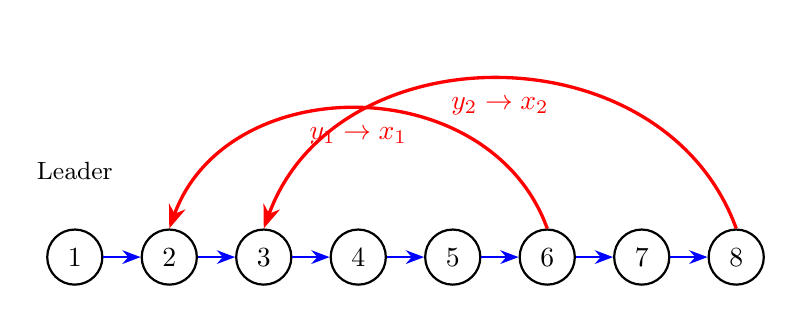
\begin{tikzpicture}[
		agent/.style={
			circle, draw, thick,
			minimum size=7mm,
			inner sep=0pt
		},
		chain/.style={-{Stealth}, thick, blue},
		reverse/.style={-{Stealth}, very thick, red}
		]
		
		% Nodes
		\foreach \i in {1,...,8}
		\node[agent] (n\i) at (1.2*\i,0) {\i};
		
		% Directed chain
		\foreach \i [evaluate=\i as \j using int(\i+1)] in {1,...,7}
		\draw[chain] (n\i) -- (n\j);
		
		% Reverse edge 6 -> 2
		\draw[reverse]
		(n6.north) to[out=110,in=70,looseness=1.15]
		node[midway,below=1mm] {\textcolor{red}{$y_1\to x_1$}}
		(n2.north);
		
		% Reverse edge 8 -> 3
		\draw[reverse]
		(n8.north) to[out=110,in=70,looseness=1.15]
		node[midway,below=1mm] {\textcolor{red}{$y_2\to x_2$}}
		(n3.north);
		
		% Leader indication
		\node[above=5mm of n1] {\small Leader};
		
	\end{tikzpicture}
	\caption{Illustration of two cycles at different topological
		positions in a directed chain. The cycle with head $x_1=3$
		is closer to the leader than the cycle with head $x_2=5$.}
	\label{fig:topological_cycle_position}
\end{figure}


The restriction in the paper by Hao et. al \cite{hao2019role} requires the longer cycle to be closer to the leader. This allows the cycle lengths to be ordered as $\ell_1>\ell_2$, so that terms such as $s^{\ell_1-\ell_2}$ appearing in the characteristic polynomial have nonnegative integer exponents. Without this restriction, such expressions may involve negative powers and would no longer constitute a polynomial in $s$, making the adopted polynomial-based analysis inapplicable in its original form. For instance, in the configuration illustrated in
Fig.~\ref{fig:topological_cycle_position}, $\ell_1=4$ and $\ell_2=5$, giving $\ell_1-\ell_2=-1$. Consequently, the
corresponding term becomes $s^{-1}$ rather than a nonnegative integer power of $s$. 

The present Chapter 2 analysis removes this restriction by considering all six possible relative arrangements of the two cycles.

Therefore, ``strictly closer'' refers to the relative ordering of the cycle head indices, subject to the longer-cycle condition, and not to any prescribed physical or numerical distance.


%\revision
%I will replace the qualitative phrase by this explicit index-based definition and state that ``strictly closer'' means a strictly smaller head-node index, not a prescribed physical distance.

\comment{Can the results in this chapter extend to graph topologies other than directed chains?}
\response
The present proofs exploit the chain's topological ordering and the fact that each reverse edge closes a uniquely identifiable interval of the chain. This structure makes the characteristic determinant reducible to the scalar polynomial equations derived in the chapter. For a general directed acyclic graph, a reverse edge can close several directed paths and hence several cycles; the same interval-based classification and scalar reduction need not apply. Some ideas may extend when the graph has a suitably simple path or parent-child structure, but this requires a separate analysis.

%\revision
%I will make the chain-topology assumption prominent in the chapter statement of scope and add a paragraph explaining that extension to general DAGs or digraphs is not automatic. Possible extensions to graphs with a unique path between the reverse-edge endpoints or restricted strongly connected components will be identified as future work.
\comment{Simulation 2.4.1: It may still be worthwhile to include the velocity plots to show transients. How is $\gamma$ chosen and why is such a precise value (4 decimal places) considered? It may be useful to check if consensus is also achieved for $\gamma$ less than this value?}

\response
Including the velocity trajectories provides a more complete illustration of the transient response and allows both position and velocity consensus to be examined. Simulation 2.4.1 in the Chapter is reproduced here as Figure \ref{Case2bconsensus}.  The value of $\gamma$ used in Simulation 2.4.1 is calculated using the analytical sufficient stability condition established in Theorem 2.26. The corresponding threshold is determined from the dominant non-zero Laplacian eigenvalue for the considered two-loop topology. Thus, the selected value is based on the theoretical stability condition rather than empirical tuning. The value is reported to four decimal places to represent the numerical evaluation of the analytical expression. This precision is for reporting purposes and does not imply that such precision is essential for practical implementation.

\begin{figure}[H]
	\centering
	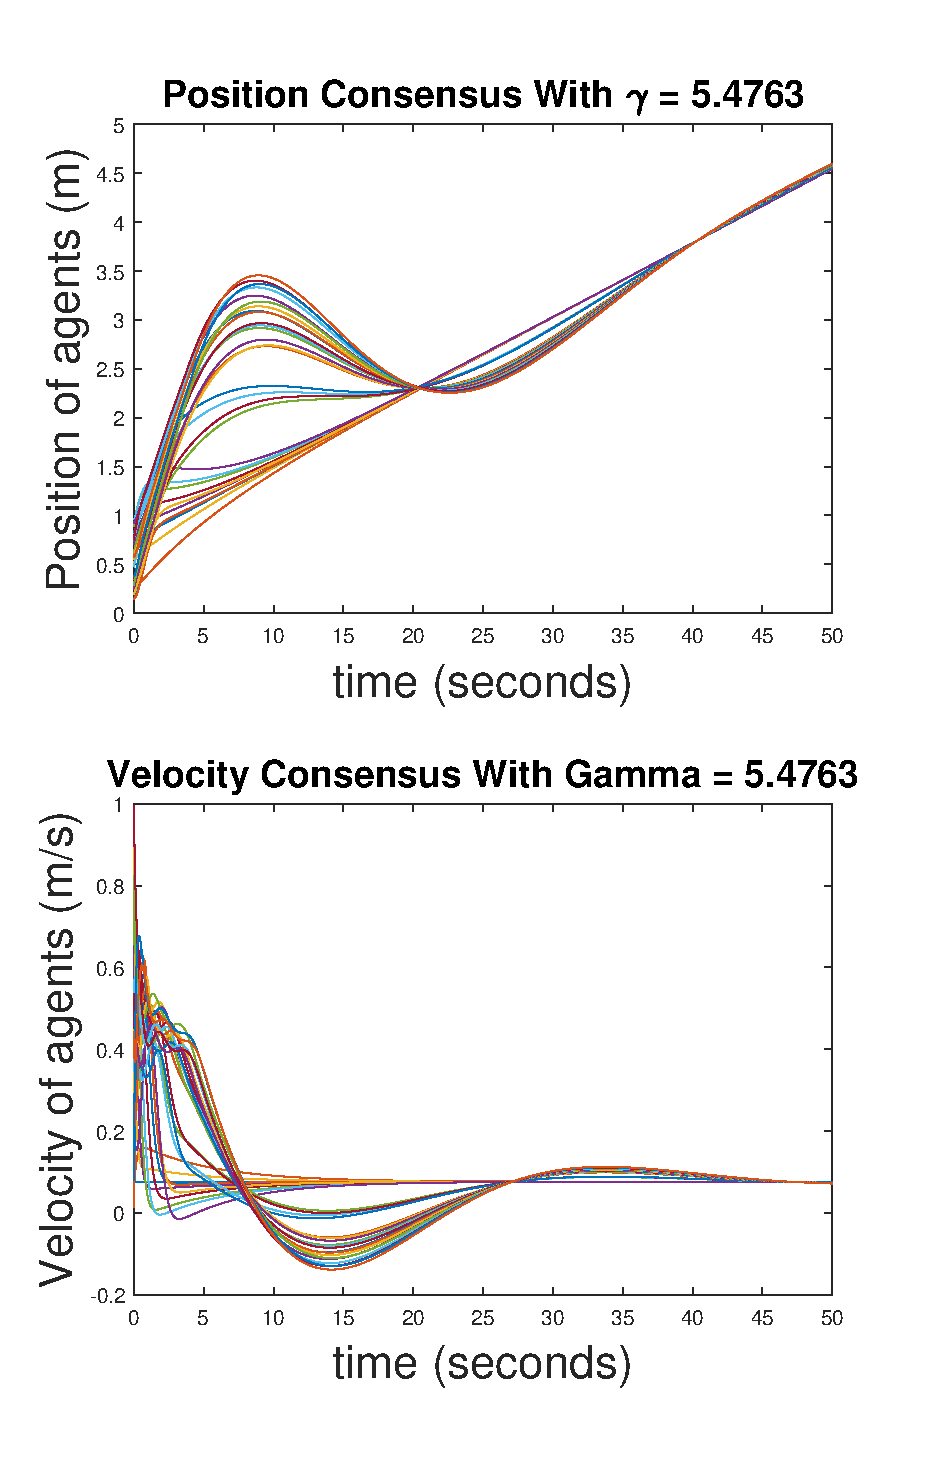
\includegraphics[width=0.75\textwidth,keepaspectratio]{2_Images/2.4.1_Position_Velocity_Combined_Sufficient_Gamma.eps}
	\caption{Position and velocity consensus in the presence of two reverse edges, where $x_1<x_2=y_1<y_2$.}
	\label{Case2bconsensus}
\end{figure}

Since the condition established in Theorem 2.26 is sufficient but not necessary, consensus may also be achieved for values of $\gamma$ below the calculated sufficient bound. This is shown in Figure \ref{Case2bconsensus_below_calculated_gamma}. 

\begin{figure}[H]
	\centering
	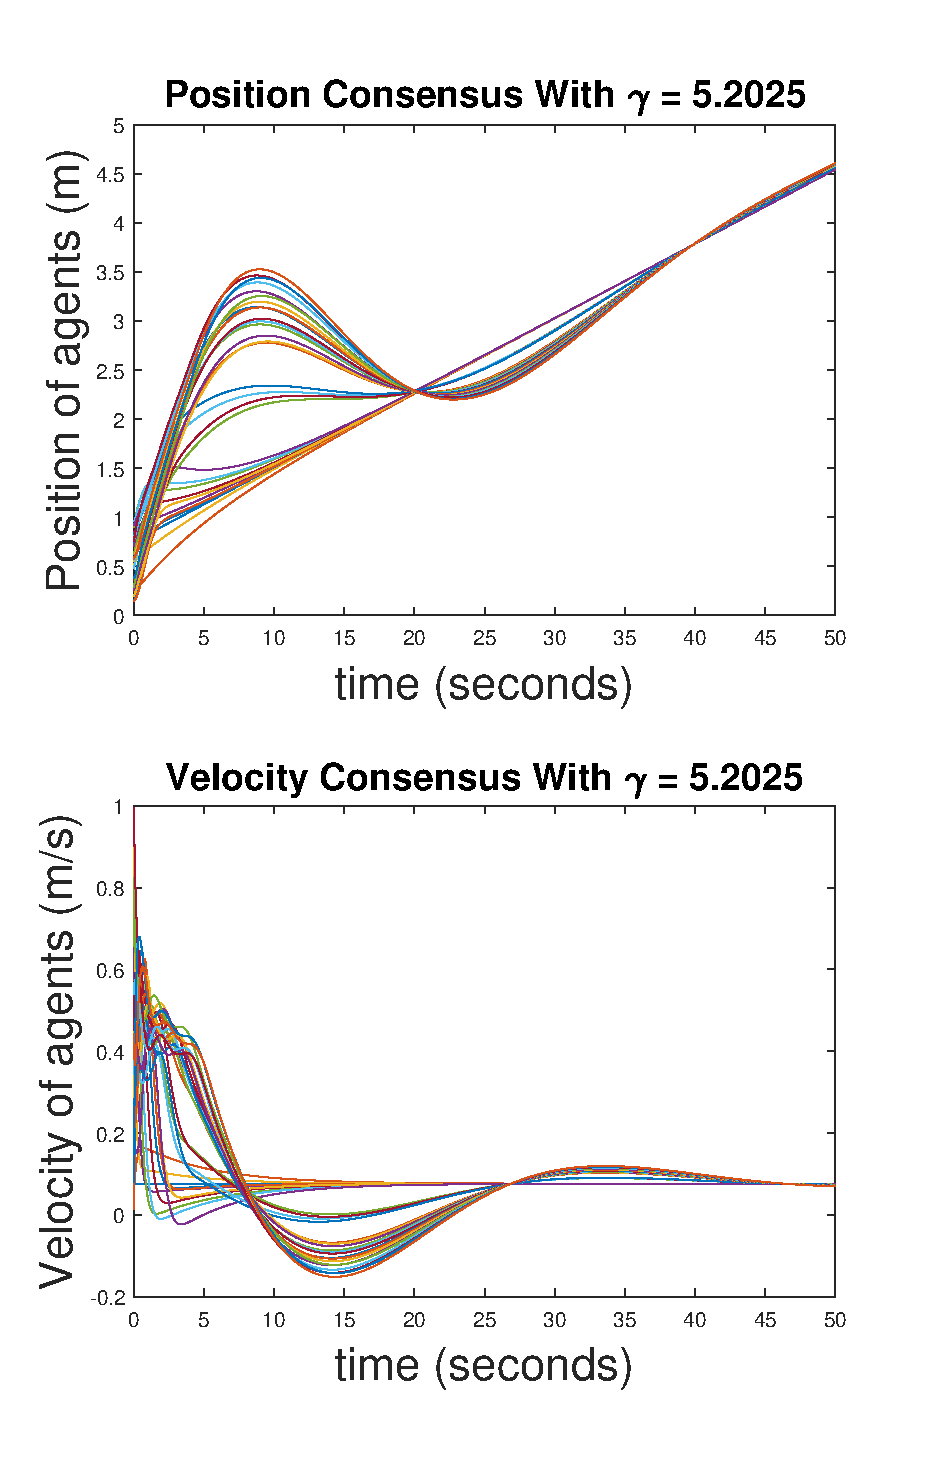
\includegraphics[width=0.75\textwidth,keepaspectratio]{2_Images/2.4.1_Position_Velocity_Combined_Below_Sufficient_Gamma.eps}
	\caption{Position and velocity responses for a velocity coupling parameter slightly below the calculated sufficient value.}
	\label{Case2bconsensus_below_calculated_gamma}
\end{figure}

 the exact stability threshold is evaluated using the necessary and sufficient condition for second-order consensus:
\begin{equation}
	\gamma_{\mathrm{stab}}
	=
	\max_{i\in\{2,\ldots,N\}}
	\left[
	\frac{|\mathfrak{Im}(\lambda_i)|}{|\lambda_i|}
	\sqrt{\frac{1}{\mathfrak{Re}(\lambda_i)}}
	\right]
	=1.7532.
\end{equation}
To examine the system response below this threshold, another simulation is performed with
\begin{equation}
	\gamma_2=0.95\gamma_{\mathrm{stab}}
	=0.95\times1.7532
	\approx 1.6655.
\end{equation}
The resulting position and velocity trajectories, shown in Fig.~\ref{Case2bconsensus_Below_Threshold}, demonstrate the breakdown of consensus.

\begin{figure}[H]
	\centering
	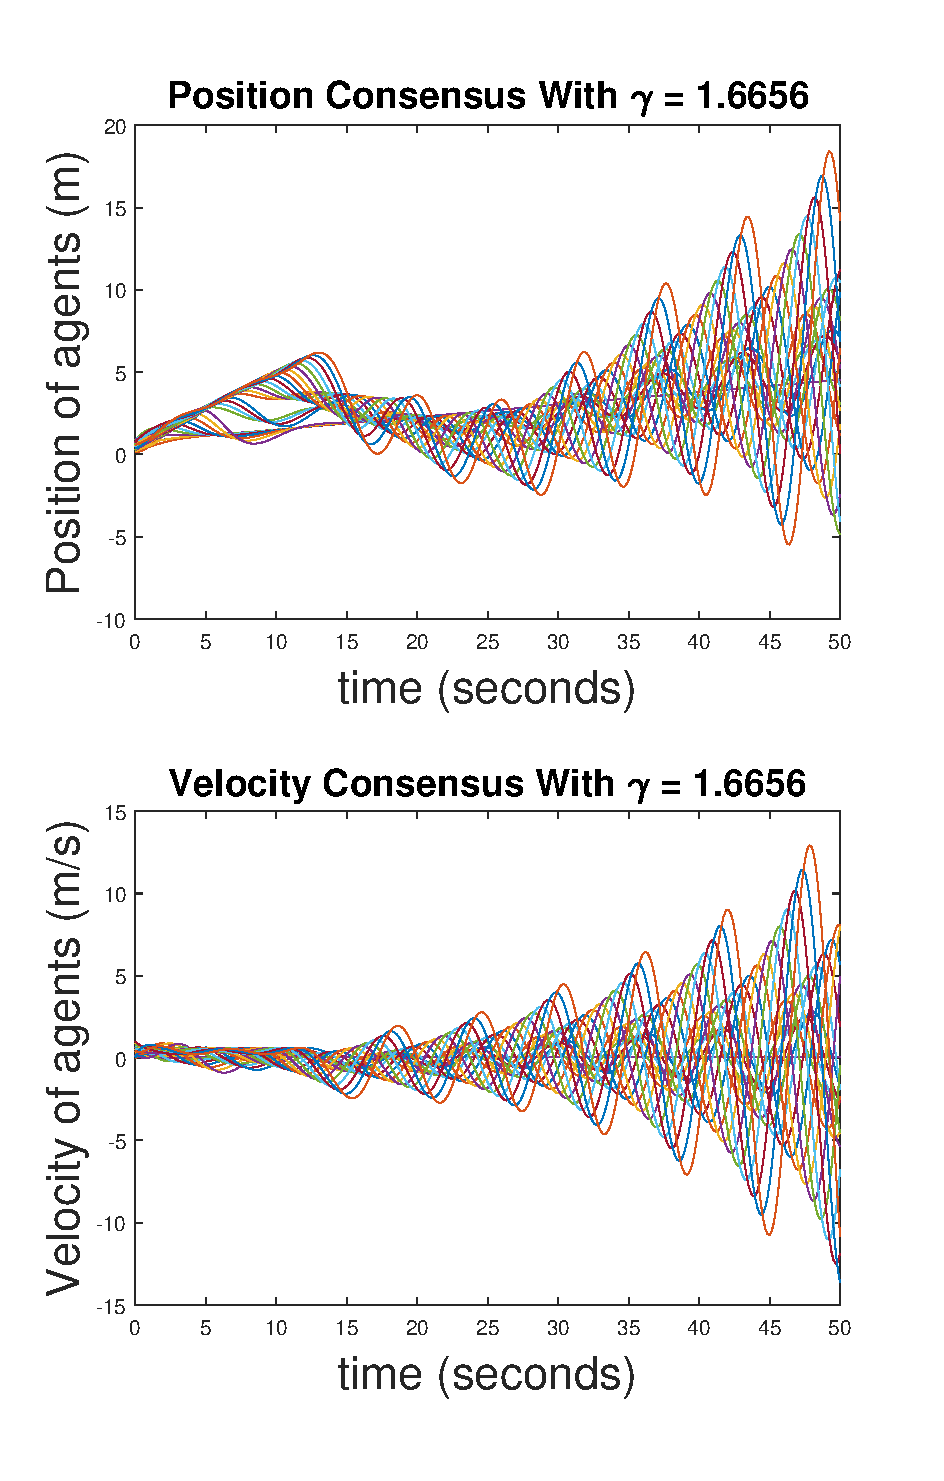
\includegraphics[width=0.75\textwidth,keepaspectratio]{2_Images/2.4.1_Position_Velocity_Combined_Below_Threshold_Gamma.eps}
	\caption{Breakdown of position and velocity consensus when the velocity coupling parameter is below the stability threshold.}
	\label{Case2bconsensus_Below_Threshold}
\end{figure}

The three simulations collectively illustrate the distinction between the sufficient coupling bound and the exact stability threshold. In particular, consensus is achieved for $\gamma=5.2025$, even though this value is below the sufficient bound of $5.4763$. However, reducing the coupling parameter below the exact stability threshold of $1.7532$ results in consensus failure. Thus, the sufficient condition provides a conservative guarantee, whereas the necessary and sufficient condition identifies the actual stability boundary for the considered network.

\revision
Figure 2.7 has been revised to include both position and velocity trajectories, thereby providing a more complete illustration of the transient response. In addition, a comparative simulation using a value of $\gamma$ below the calculated sufficient coupling parameter has been included in Figure 2.8 to investigate whether consensus can still be achieved below this bound.

Furthermore, the necessary and sufficient stability condition has been used to determine the exact stability threshold for the considered topology. A simulation with $\gamma$ below this threshold has been included in Figure 2.9 to demonstrate the resulting breakdown of consensus.


\comment{The time axis of Fig. 2.8 may be shortened to say 25 seconds to reveal more details about the transients.}

\response
The transient response depends on the initial position and velocity conditions of the agents. The original time horizon was selected to illustrate the overall convergence behaviour. However, to provide a clearer view of the transient dynamics, Figure 2.8 has been regenerated using appropriately selected initial conditions and reproduced here as Figure \ref{Case3cconsensus}

	\begin{figure}[H]
	\centering
	%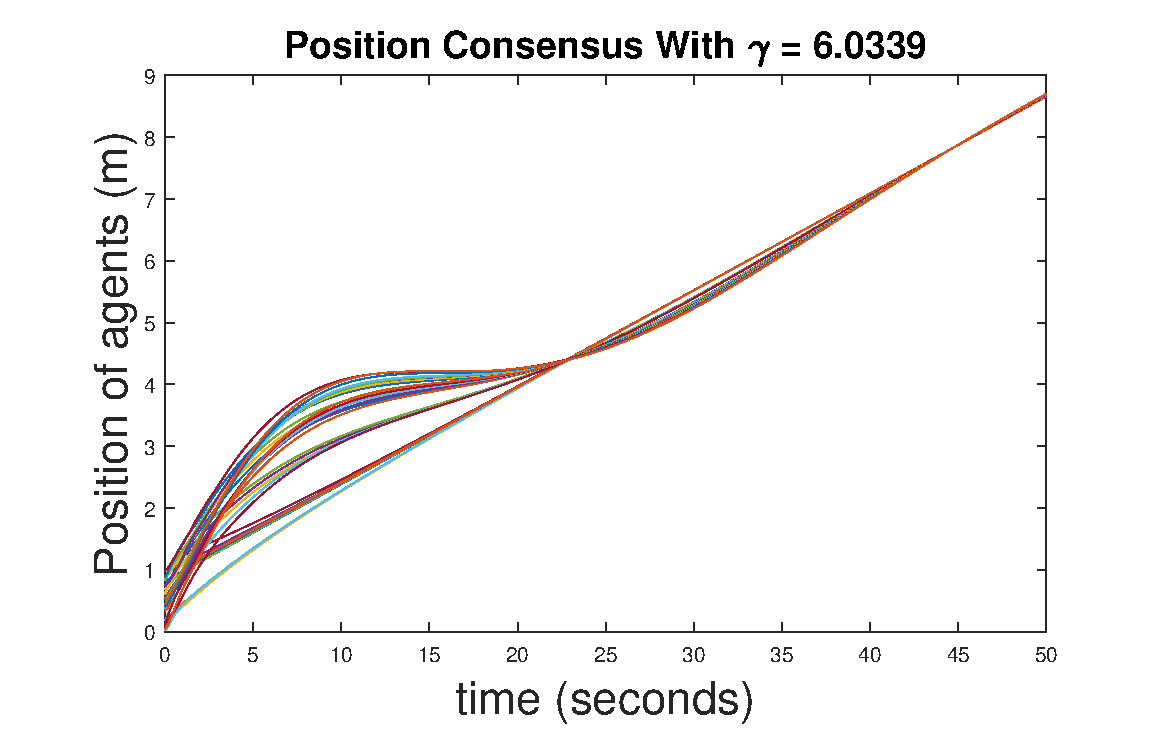
\includegraphics[width=0.75\textwidth,keepaspectratio]{2_Images/position_plot_for_theis.eps}
	%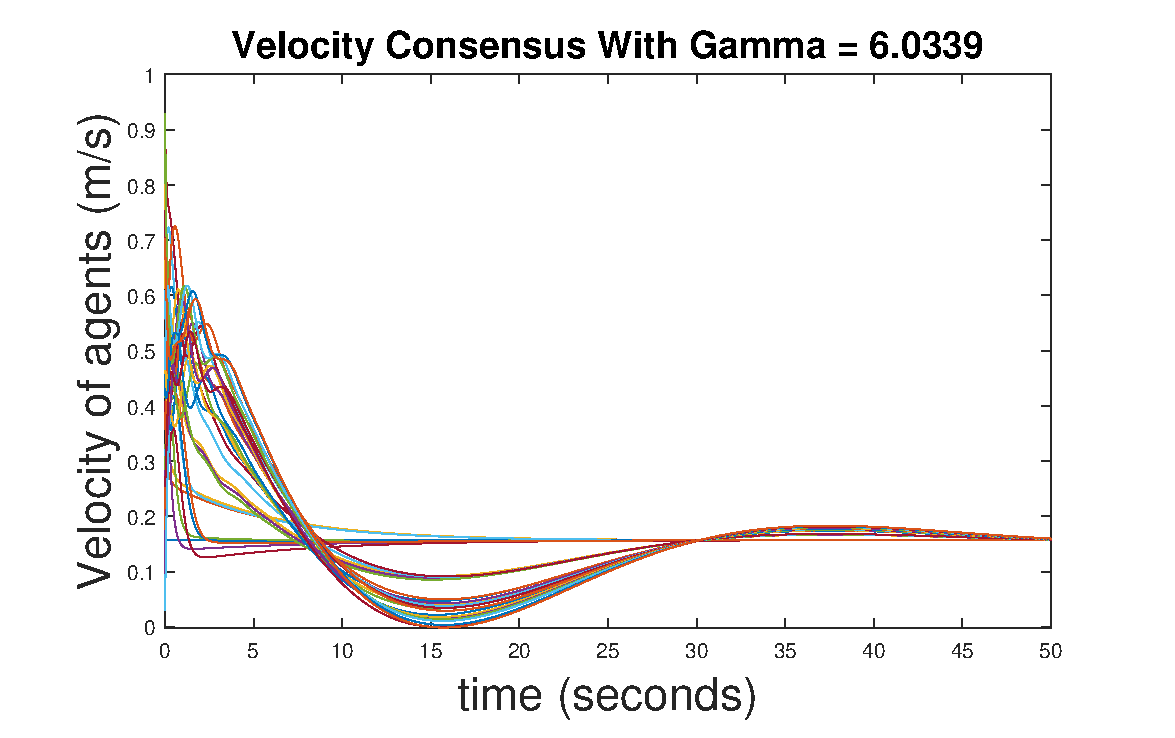
\includegraphics[width=0.75\textwidth,keepaspectratio]{2_Images/velocity_plot_for_theis.eps}
	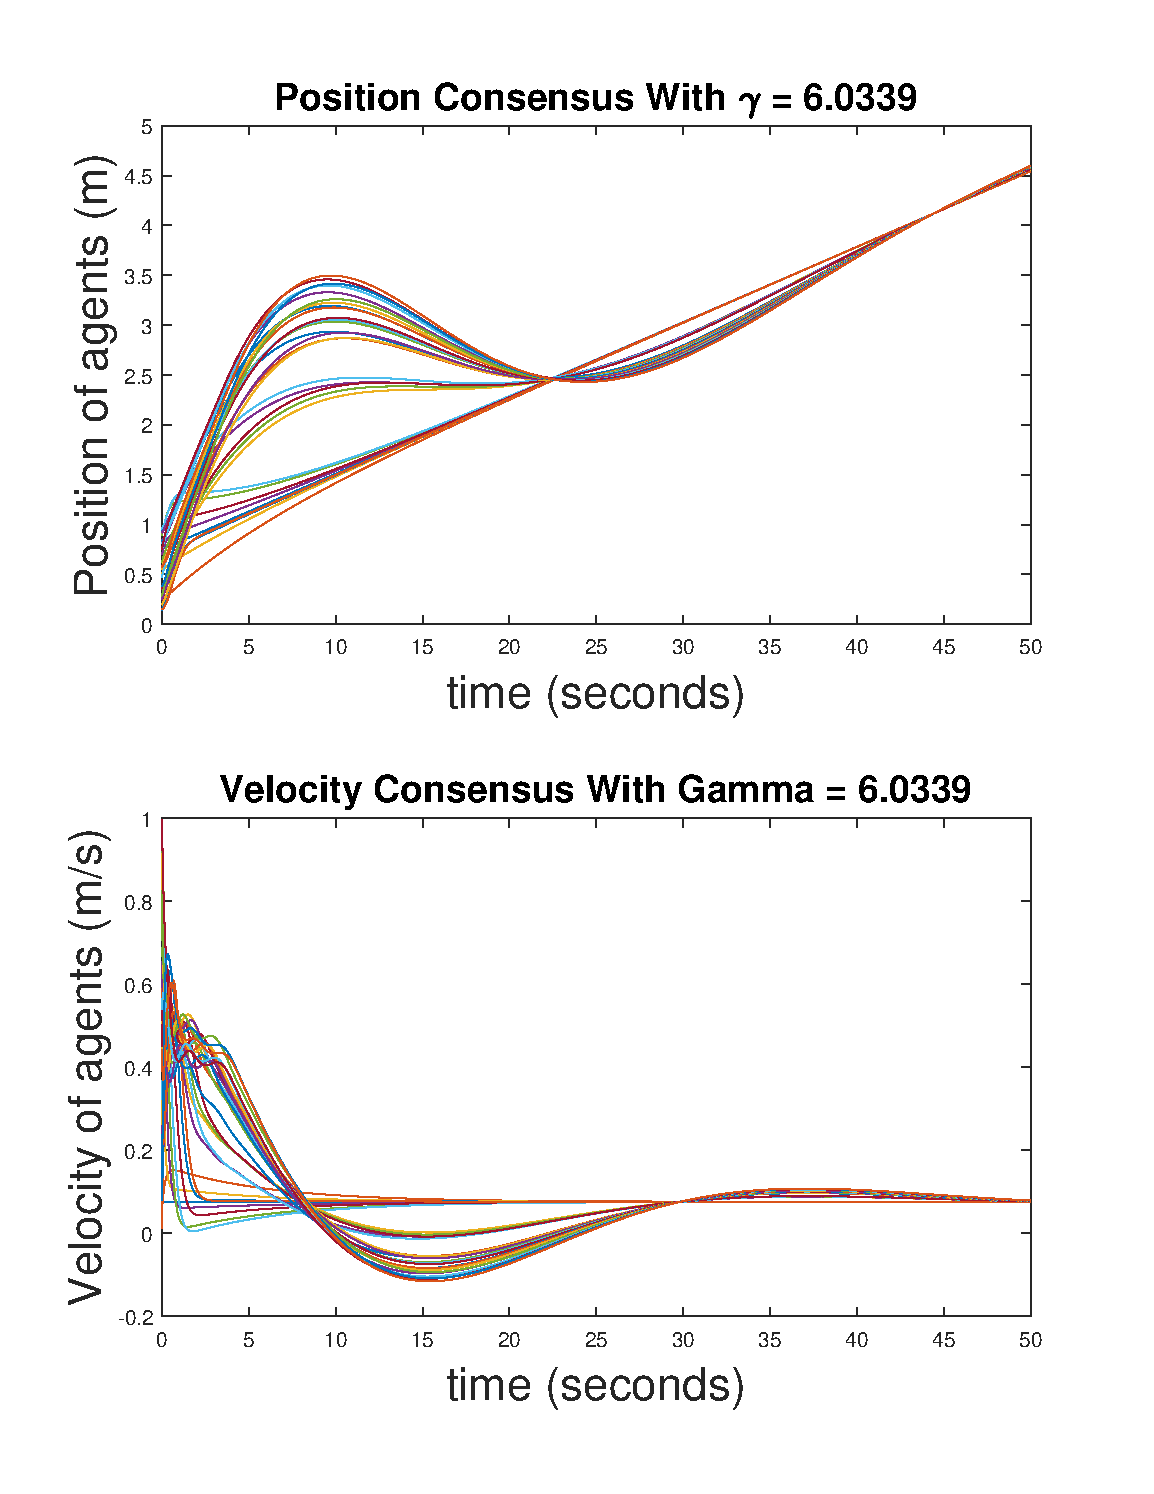
\includegraphics[width=0.7\textwidth,keepaspectratio]{2_Images/New_Stable.eps}
	\caption{Position and Velocity consensus in presence of two reverse edges where $x_1<x_2<y_1<y_2$}
	\label{Case3cconsensus}
\end{figure}

\revision
Figure 2.8 (renumbered as Figure 2.10 in the revised thesis) has been regenerated with suitably selected initial conditions. This provides a clearer illustration of the transient convergence behavior of the agents.

\comment{Is it possible to simulate the consensus collapse that you describe in Section 4.8?}
\response
I understand this comment refers to the consensus collapse. Figure 2.9 \& Figure 2.11 (here reproduced as Figure \ref{Case2bconsensus_Below_Threshold} \& Figure \ref{Case3cconsensusBreakdown}) has been included to illustrate the breakdown of consensus under the considered conditions.

\begin{figure}[H]
	\centering
	%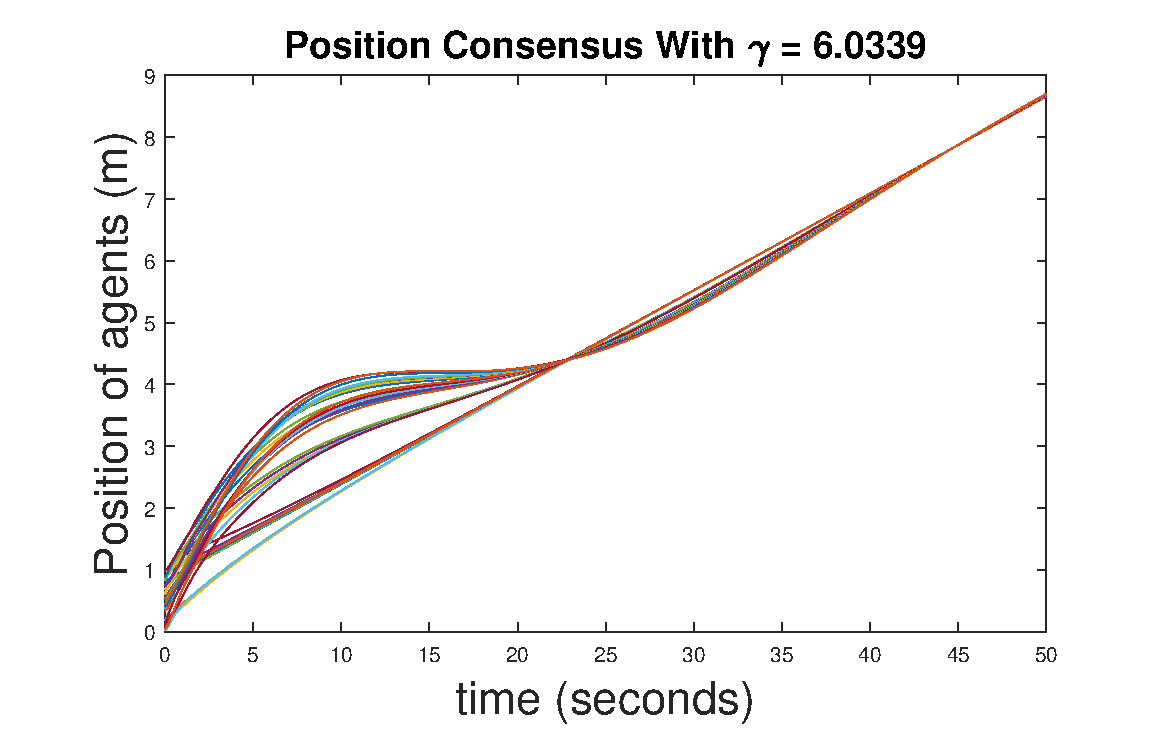
\includegraphics[width=0.75\textwidth,keepaspectratio]{2_Images/position_plot_for_theis.eps}
	%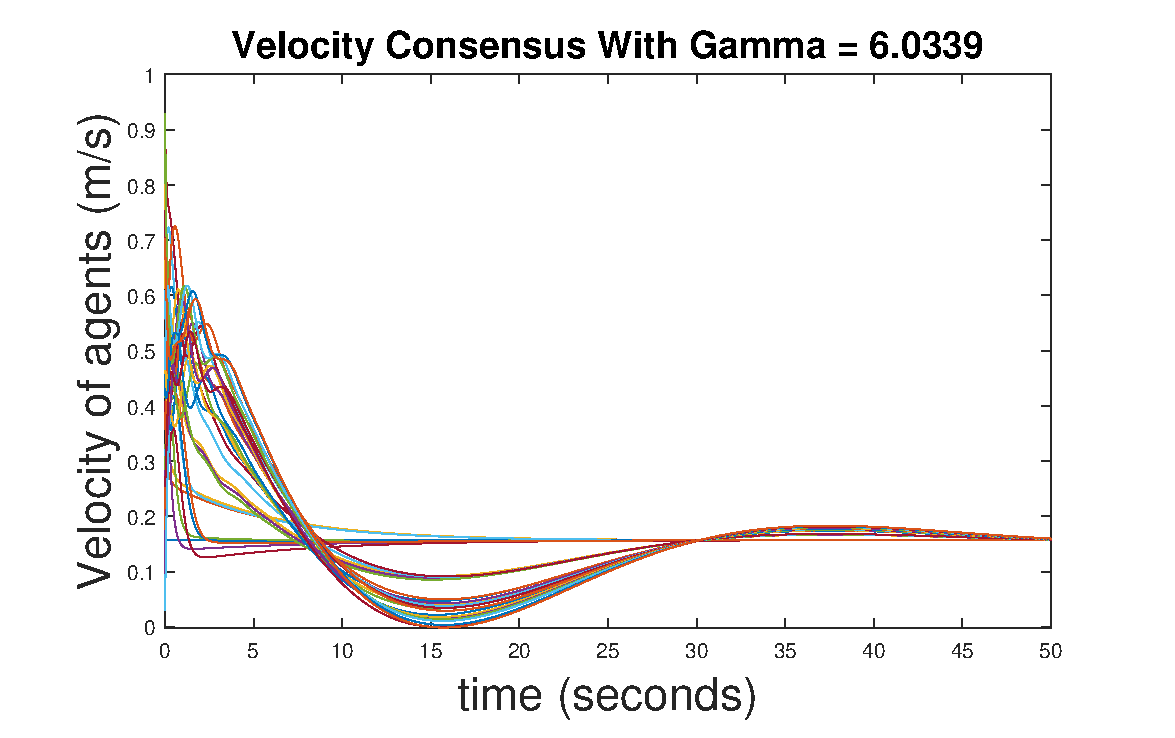
\includegraphics[width=0.75\textwidth,keepaspectratio]{2_Images/velocity_plot_for_theis.eps}
	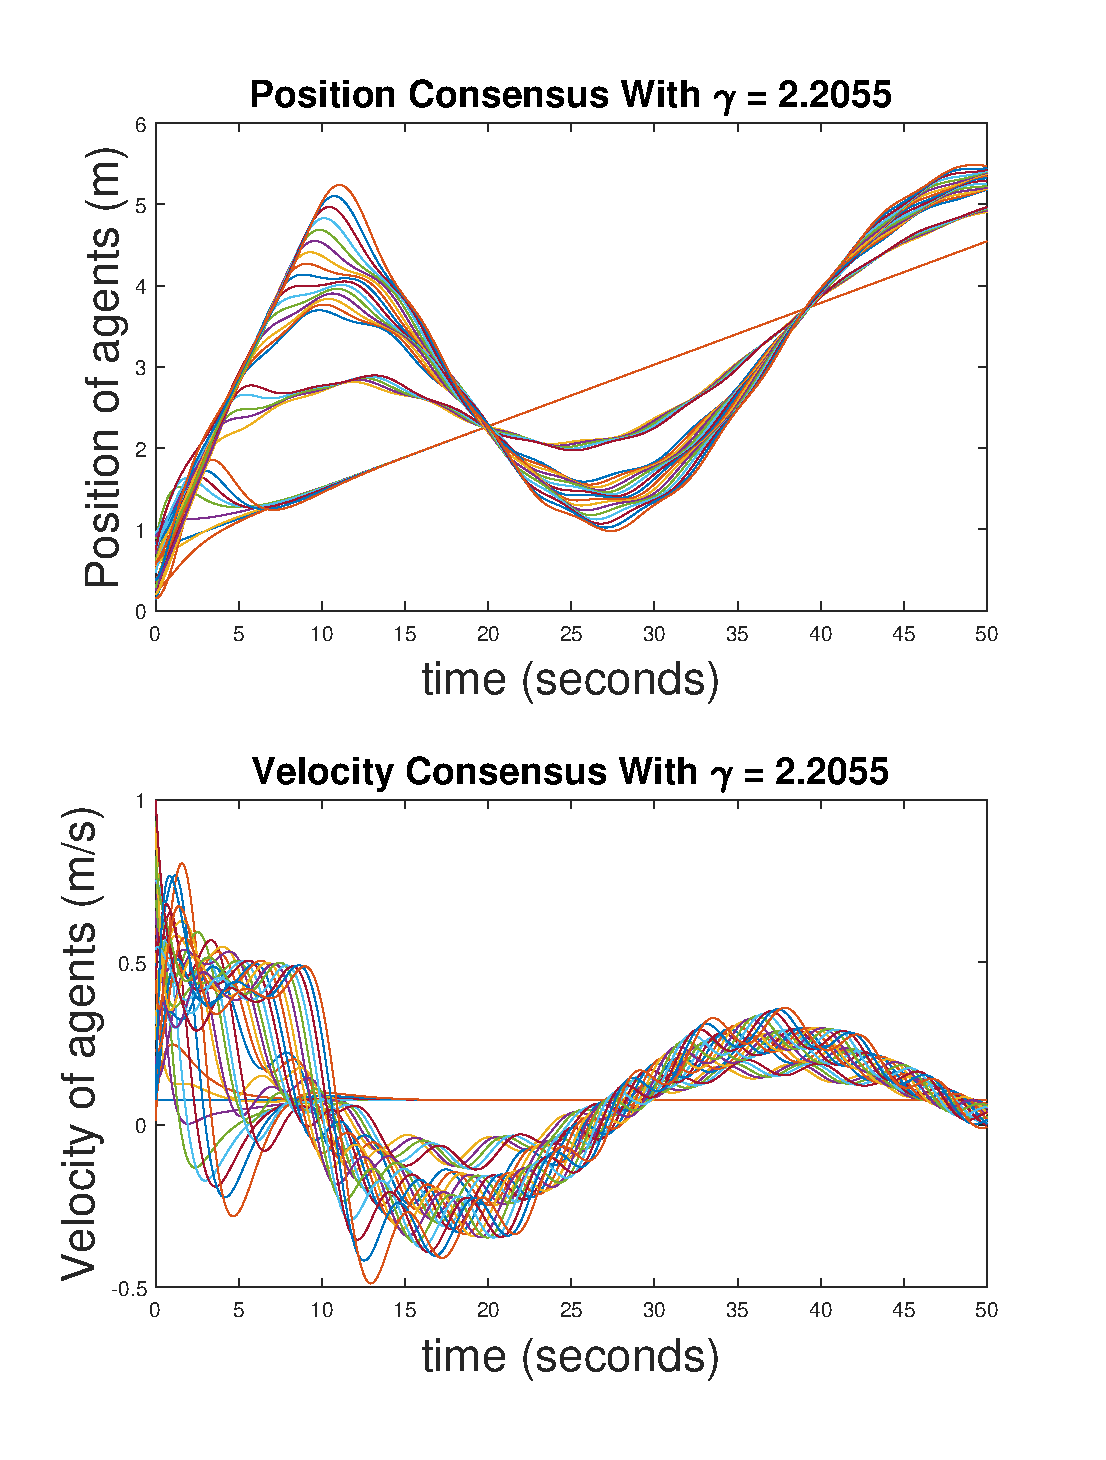
\includegraphics[width=0.75\textwidth,keepaspectratio]{2_Images/New_Unstable.eps}
	\caption{Consensus Breakdown in presence of two reverse edges where $x_1<x_2<y_1<y_2$}
	\label{Case3cconsensusBreakdown}
\end{figure}

\subsection*{Chapter 3}

\comment{What is the effect of node/edge scaling on performance or the rate at which consensus is achieved? Similarly, it may be worthwhile to study the effect of scaling on robustness to disturbances and noise ($\mathcal{H}_2$-norm?).}
\response
The scaling constructions in Chapter 3 are designed to move the relevant Gershgorin regions and increase a lower bound on the real parts of the nonzero eigenvalues, thereby restoring stability for a fixed $\gamma$. A larger guaranteed spectral separation generally improves the asymptotic convergence-rate bound, although the actual dominant eigenvalue and transient response depend on the complete scaled Laplacian. The chapter's proofs establish stability, not an optimal transient-performance design. Similarly, the $\mathcal{H}_2$ results in Chapter 4 are derived for a different, undirected path-graph setting; they do not directly quantify the $\mathcal{H}_2$ effect of the directed node/edge scaling in Chapter 3.

%\revision
%I will add a discussion explaining the distinction between (i) the stability guarantee supplied by the Gershgorin's separation, (ii) the convergence rate governed by the actual dominant eigenvalue, and (iii) disturbance/noise amplification, which requires a separate input-output analysis. A quantitative $\mathcal{H}_2$ comparison for the scaled directed networks will be identified as future work rather than inferred from the existing Chapter 4 formula.

\comment{Does the scaling method work for arbitrary feedback-loop range? How does it scale with increase in this range?}
\response
For the leader-excluded single-loop case treated by the node-scaling theorem, the construction is stated for loop range $\ell=y_1-x_1$ and any fixed $\gamma>0$. The minimum initial scaling level satisfies
\[
p_1 \geq \frac{\ell+1}{\gamma^2}+\varepsilon,\qquad \varepsilon>0,
\]
and the scaling factors are arranged as an arithmetic progression. Thus, for fixed $\gamma$, the required baseline scaling grows linearly with $\ell+1$. The edge-scaling and combined-scaling constructions have analogous range-dependent design inequalities. The root-node loop is a distinct case and is handled by the complementary root-locus construction, not by simply applying the leader-excluded node-scaling theorem.


\comment{It may be worthwhile to analyze the root-locus-based methods for robustness to modelling errors.}
\response
The root-locus construction in Section 3.4 provides a nominal gain margin for the selected complementary transfer function and design parameters. This is useful as a first robustness indicator with respect to gain variation in that scalar loop representation. It does not, however, constitute a complete robustness analysis for simultaneous uncertainty in edge weights, agent dynamics, delays, or unmodeled dynamics. In particular, a classical root-locus gain margin should not be interpreted as a structured uncertainty bound for the full network.

%\revision
%I will clarify this distinction and state that the computed gain margin can be used to select a nominal design with some gain-variation tolerance. Robustness to structured plant and graph uncertainty, including worst-case pole migration, remains a separate extension requiring an uncertainty model and an appropriate robust-control analysis.

\subsection*{Chapter 4}
	
\comment{Any reason for moving to undirected graphs? Do the results extend trivially to directed graphs?}
\response
The original motivation was to investigate disturbance attenuation and $\mathcal{H}_2$ performance in directed networks. However, during the course of this investigation, it became evident that even the undirected case, particularly the effect of cycle placement and overlap on $\mathcal{H}_2$ performance, had not been explored fully. Addressing this question itself led to several interesting results, which form the contribution of Chapter 4.

The restriction to undirected graphs is also mathematically significant. The analysis in this chapter exploits the symmetry of the graph Laplacian and the resulting positive-definite structure of the essential edge Laplacian. These properties enable the reduced-order dynamics and the associated Lyapunov equation to be handled analytically. For directed graphs, the loss of symmetry makes the corresponding analysis considerably more complicated, and the techniques developed here cannot be directly extended. In particular, extending the analysis to directed cyclic graphs may require a substantial reconsideration of the mathematical tools and is beyond the scope of the present work.

%\revision
%I will clarify the original motivation for studying directed networks, explain why the investigation focused on the less-explored undirected case, and explicitly identify the extension to directed cyclic graphs as an important direction for future research.

\comment{Please substantiate the statement ``In practical deployments, edge communication channels are corrupted by zero-mean Gaussian measurement noise''. Is this true in general?}
\response
The statement should not be interpreted as a universal empirical description of communication-channel errors. Rather, the
zero-mean Gaussian white-noise model is adopted as a standard stochastic representation of measurement uncertainty in consensus networks. For example, Zelazo and Mesbahi developed an edge-based $\mathcal{H}_2$ framework for noisy consensus in which both process disturbances and relative-measurement noise are modelled as Gaussian white-noise inputs~\cite{zelazo2009h2}. Their subsequent work with Schuler and Allgöwer used this framework to investigate the influence of cycle structure on network performance, considering disturbances entering through both the process and measurement channels~\cite{zelazo2013performance}. Similarly, Young, Scardovi, and Leonard studied the robustness
of consensus under white-noise disturbances and communication noise, including directed communication topologies
\cite{young2010robustness}.

This modelling choice is appropriate for the present investigation for three reasons. First, zero-mean noise represents measurement fluctuations around an unbiased relative-state estimate, without introducing a systematic measurement bias. Second, the white-noise assumption provides an idealization of rapidly varying measurement errors whose correlation time is short relative to the network dynamics. Third, the Gaussian assumption provides a convenient stochastic representation of aggregate measurement and estimation uncertainties. Together with the assumption of mutually uncorrelated noise sources, this yields a tractable model for analysing the mean-square disagreement through the $\mathcal{H}_2$ norm.

It is important to note that the $\mathcal{H}_2$ analysis relies on the second-order noise statistics and the white-noise assumption; Gaussianity itself is not essential to the covariance-based $\mathcal{H}_2$ calculation. In practical systems, measurement errors may also exhibit bias, temporal or spatial correlation, quantization, and packet losses. These effects are not explicitly represented in the present model and would require appropriate extensions.

%\revision
%I will revise the statement to clarify that zero-mean Gaussian white noise is a modelling assumption adopted for the stochastic performance analysis, rather than a universal property of practical communication channels. I will also cite the relevant noisy-consensus literature, particularly the edge-based formulation of Zelazo and Mesbahi and subsequent work on noisy consensus networks, and explain the rationale and limitations of the adopted assumptions.


\comment{Why call (4.10) uncoupled global state equations?}
\response
I agree that ``uncoupled'' is inaccurate. Although the equations are written in global stacked coordinates, the agents remain dynamically coupled through the graph Laplacian $\mathcal{L}$:
\[
\dot{x}=v,\qquad \dot{v}=-\mathcal{L}x-\gamma \mathcal{L}v+q-Er.
\]
The word was intended to indicate that the equations are expressed at the global nodal level before the subsequent edge-coordinate transformation, not that the individual agents are independent.

\revision
``uncoupled global state equations'' has been replaced with ``global nodal state equations'' (or ``network-level state equations'') throughout the relevant discussion.

\comment{The standard $\mathcal{H}_2$ norm is defined for white-noise processes. Based on the problem definition in this chapter, the process and measurement noise are not necessarily white. Is there a case for whitening the noise for the conditions of the $\mathcal{H}_2$ norm to be satisfied?}
\response
The analysis does not involve whitening the physical disturbances. Instead, the process and measurement disturbances are modeled as zero-mean white-noise inputs from the outset. This assumption is explicitly specified in the problem formulation through their covariance relations:
\[
\mathbb{E}[q_i(t)q_i(\tau)]
=\sigma_q^2\delta(t-\tau),
\qquad
\mathbb{E}[r_{ij}(t)r_{ij}(\tau)]
=\sigma_r^2\delta(t-\tau).
\]
Thus, the derivation of the $\mathcal{H}_2$ performance measure in this chapter is conditional on the adopted white-noise model.

This modeling approach is consistent with established literature on noisy consensus networks. For instance, Zelazo and Mesbahi (2009) developed an edge-based $\mathcal{H}_2$ framework for agreement protocols under noise \cite{zelazo2009h2}, while Young, Scardovi, and Leonard (2010) investigated the robustness of consensus networks under directed communication by modeling the disturbances as white-noise inputs \cite{young2010robustness}. These works provide a relevant foundation for adopting the white-noise model in the present analysis.

The white-noise assumption provides a tractable representation of rapidly varying stochastic disturbances and allows the steady-state mean-square disagreement to be quantified through the $\mathcal{H}_2$ norm and the associated Lyapunov equation. The Gaussian assumption is additionally adopted for the stochastic disturbance model, although the covariance-based $\mathcal{H}_2$ calculation itself does not require Gaussianity.

If the actual disturbances exhibit significant temporal correlation, a more general analysis would require an appropriate coloured-noise model, for example, through stable shaping filters and an augmented state-space realization. Such an extension is not considered in the present work.

%\revision
%I will clarify that the process and measurement disturbances are explicitly assumed to be white in the problem formulation, rather than being whitened as a preprocessing step. I will strengthen the justification by citing established noisy-consensus literature and state that the derived $\mathcal{H}_2$ results are conditional on the adopted white-noise model.

\comment{Why restrict analysis to path graphs? Do the results hold in general for all cyclic graphs or only a class of cyclic graphs?}
\response
The path graph is selected because it provides a canonical one-dimensional structure in which the location, length, and overlap of added cycles can be parameterized explicitly. This enables the derivation of closed-form expressions for the $\mathcal{H}_2$ norm and the corresponding optimal cycle-placement and overlap conditions.

Nevertheless, the considered topology has connections to other network structures. For example, a ring network can be represented as a path graph with an additional edge connecting its two endpoints and is therefore a special case of the cyclic topologies considered in this chapter. Similarly, consider a rooted parent--child tree in which communication links are directed from parent to child. Adding an undirected communication link between two nodes creates a cycle along the unique path connecting them. Such networks provide a natural setting for extending the present edge-based analysis.

However, the closed-form expressions and optimal results derived in this chapter rely on the specific path structure. In a branched parent--child network, additional branches can influence the network dynamics and the resulting $\mathcal{H}_2$ performance. Consequently, the present results cannot be directly generalized to arbitrary cyclic graphs, and the corresponding performance and optimal conditions require further analysis.

%\revision
%I will include illustrative examples of a ring network and a branched parent--child network with an additional communication link. I will clarify that the ring topology is directly covered by the present formulation, whereas the parent--child network illustrates a possible extension of the edge-based analysis. The scope of the established closed-form results will remain restricted to the path-based cyclic topologies considered in this chapter.

\subsection*{Chapter 5}

\comment{Is it possible to accommodate moving targets using this or a similar scheme?}
\response
The present Chapter 5 construction assumes a stationary target, with the engagement geometry and terminal conditions defined with respect to a fixed target location. Extending the formulation to moving targets is not straightforward. Even for a non-maneuvering target with constant velocity, the interception time becomes an additional unknown, and the terminal impact angle must be defined as the angle between the missile's and target's velocity vectors at the instant of interception. Consequently, both the interception condition and the terminal engagement geometry would need to be reformulated.

For a manoeuvring target, predicting its position and velocity at the interception instant introduces further challenges. Although the underlying path-construction approach may provide a starting point for investigating this problem, its applicability under the modified terminal conditions and the associated path-feasibility constraints would require a separate analysis.

Therefore, moving-target interception is identified as a possible extension of the present work and is not covered by the results established in this chapter.

%\revision
%I will explicitly state the stationary-target assumption and identify moving-target interception as a possible extension, highlighting the need to reformulate the interception-time and terminal impact-angle conditions.

\comment{The current theory assumes a fixed design radius and does not provide stability or continuity guarantees for continuously varying $r_d$, whereas you propose adjusting the secondary turn radius $r_d$ to satisfy simultaneous terminal approach angle and time-of-arrival constraints. Can $r_d$ be updated online while preserving continuity and terminal guarantees?}
\response
In the submitted Chapter 5 analysis, $r_d$ is treated as a fixed path-design parameter selected from a feasible interval. The monotonicity and continuity argument establishes the existence and uniqueness of a fixed $r_d^\star$ for a feasible requested arrival time. The closed-loop implementation then tracks the resulting precomputed geometry. However, the present analysis does not establish stability, continuity, or terminal guarantees when $r_d$ is continuously varied online.

Online adaptation of $r_d$ while preserving path continuity and satisfying the terminal approach-angle and time-of-arrival
constraints is an interesting but challenging extension. It would require a separate analysis of the parameter-update mechanism, geometric feasibility, and closed-loop guarantees. This is beyond the scope of the present work.

%\revision
%I will clarify that the theoretical guarantees in Chapter 5 apply to a fixed selected value of $r_d^\star$. I will also identify online adaptation of $r_d$, with preservation of path continuity and terminal constraints, as an important direction for future research in the concluding chapter.

\subsection*{Chapter 6}

\comment{It would be useful to include details on why spiral guidance is intrinsically better than the Dubins-based method.}
\response
The advantage of the spiral-based construction over the Dubins-based
method is primarily related to the smoothness and flexibility of the
resulting trajectory, rather than universal superiority.

A classical Dubins path is composed of circular arcs and straight-line
segments. Although the trajectory is continuous and has a continuous
tangent direction (i.e., it is generally $C^1$), its curvature is
piecewise constant and changes discontinuously at the junctions
between these segments. Consequently, the trajectory is generally
not $C^2$ at these junctions. Since the lateral acceleration required
to follow a path is given by
\[
a_{\mathrm{lat}}=v^2\kappa=\frac{v^2}{r},
\]
where $v$ is the vehicle speed and $\kappa$ is the path curvature,
these curvature discontinuities can also result in discontinuities
in the lateral-acceleration demand, even when the speed is continuous.

In contrast, the Archimedean-spiral construction considered in
Chapter 6 provides continuously varying curvature. This results
in a smoother lateral-acceleration profile and avoids the abrupt
changes in acceleration demand associated with the transitions
between straight and circular segments in a classical Dubins path.
Furthermore, for the parameter range considered in this chapter,
the curvature tends to zero as the target is approached, thereby
providing a smooth terminal transition.

Another motivation for investigating the spiral-based construction
was its richer geometric structure, which offers potential flexibility
for coordinating multiple trajectories in a salvo attack scenario.
Although the present chapter focuses on individual trajectory
generation and impact-angle tracking, this flexibility motivates
further investigation of spiral-based guidance for coordinated
multi-vehicle engagements.

It is important to note that the two constructions address different
design objectives. The Dubins-like construction in Chapter 5 provides
an explicit design parameter $r_d$ for simultaneous impact-angle and
impact-time tuning, whereas Chapter 6 focuses on curvature feasibility
and impact-angle tracking. Thus, the spiral-based construction offers
advantages in trajectory smoothness and potential multi-trajectory
coordination, while the Dubins-like construction provides a direct
mechanism for space--time tuning.

%\revision
%I will strengthen the comparison in Chapter 6 by explaining thecontinuity properties of the Dubins trajectory and their implications for curvature and lateral-acceleration demand. I will also highlight the smoother curvature profile of the spiral construction and include its potential for coordinated salvo attacks as a motivation for further research. The comparison will clarify the distinct design objectives addressed by the two methods rather than claim that one is universally superior.

\comment{Sensitivity of the $\alpha$ threshold to uncertainties in speed, target positions, etc.?}
\response
The feasibility threshold in Chapter 6 is determined by the
relationship
\[
\alpha_{\mathrm{ref}}=\frac{v_p^2 f(\beta)}{a_{\max}}.
\]
Therefore, its sensitivity to variations in missile speed and
maximum available acceleration can be examined analytically.
For fixed $\beta$, the first-order relative variation is
\[
\frac{\delta\alpha_{\mathrm{ref}}}{\alpha_{\mathrm{ref}}}
\simeq
2\frac{\delta v_p}{v_p}
-\frac{\delta a_{\max}}{a_{\max}}.
\]
This indicates that the threshold is quadratically dependent on
missile speed and inversely dependent on the available acceleration.

Uncertainty in the initial target geometry affects the initial
scaling parameter $\alpha_0$, rather than directly affecting
$\alpha_{\mathrm{ref}}$. Consequently, such uncertainty changes
the feasibility margin between $\alpha_{\mathrm{ref}}$ and
$\alpha_0$.

These relations provide a local analytical sensitivity
characterization around the nominal parameter values. However,
they do not establish robustness guarantees under bounded or
stochastic uncertainties. A systematic robustness analysis
accounting for uncertainties in the engagement parameters is
beyond the scope of the present work.

%\revision
%I will clarify the dependence of the feasibility threshold on missile speed and acceleration capability, distinguish it from the influence of initial geometric uncertainty, and identify a comprehensive uncertainty and robustness analysis as a direction for future investigation.
\vspace{10pt}

\vspace{10pt}
\hrule
\vspace{8pt}
I again thank both examiners for their constructive comments, careful
evaluation, and valuable suggestions. I will incorporate the clarifications
and revisions described above and ensure that any additional numerical
results are included only after due verification.

\vspace{14pt}
Sincerely,\\[18pt]
\textbf{Avinash Kumar Dubey}\\
Roll No. 184076010\\
Department of Electrical Engineering\\
Indian Institute of Technology Bombay

\clearpage
\begin{thebibliography}{99}
\bibitem{horn2012matrix}
R. A. Horn and C. R. Johnson,
\textit{Matrix Analysis},
2nd ed., Cambridge University Press, Cambridge, 2012.

\bibitem{harville1997}
D. A. Harville,
\textit{Matrix Algebra From a Statistician's Perspective},
Springer-Verlag, New York, 1997.

\bibitem{hao2019role}
Y. Hao, Q. Wang, Z. Duan, and G. Chen,
``The Role of Reverse Edges on Consensus Performance of Chain Networks,''
\textit{IEEE Transactions on Systems, Man, and Cybernetics: Systems},
vol. 51, no. 3, pp. 1757--1765, 2021.

\bibitem{olfati2004consensus}
R. Olfati-Saber and R. M. Murray,
``Consensus problems in networks of agents with switching topology
and time-delays,''
\textit{IEEE Transactions on Automatic Control},
vol. 49, no. 9, pp. 1520--1533, 2004.

\bibitem{jadbabaie2003coordination}
A. Jadbabaie, J. Lin, and A. S. Morse,
``Coordination of groups of mobile autonomous agents using
nearest neighbor rules,''
\textit{IEEE Transactions on Automatic Control},
vol. 48, no. 6, pp. 988--1001, 2003.

\bibitem{ren2005secondorder}
W. Ren and E. Atkins,
``Second-order consensus protocols in multiple vehicle systems
with local interactions,''
in \textit{Proceedings of the AIAA Guidance, Navigation, and
	Control Conference and Exhibit}, San Francisco, CA, 2005,
Paper AIAA 2005-6238.

\bibitem{ren2007distributed}
W. Ren and E. Atkins,
``Distributed multi-vehicle coordinated control via local
information exchange,''
\textit{International Journal of Robust and Nonlinear Control},
vol. 17, pp. 1002--1033, 2007.

\bibitem{ren2008doubleintegrator}
W. Ren,
``On consensus algorithms for double-integrator dynamics,''
\textit{IEEE Transactions on Automatic Control},
vol. 53, no. 6, pp. 1503--1509, 2008.

\bibitem{dullerud2000course}
G. E. Dullerud and F. Paganini,
\textit{A Course in Robust Control Theory: A Convex Approach},
Texts in Applied Mathematics, vol. 36,
Springer-Verlag, New York, 2000.

\bibitem{zelazo2009h2}
D. Zelazo and M. Mesbahi,
``$\mathcal{H}_2$ Performance of Agreement Protocol with Noise:
An Edge Based Approach,''
in \textit{Proceedings of the 48th IEEE Conference on Decision
	and Control and 28th Chinese Control Conference},
pp. 4747--4752, 2009.

\bibitem{zelazo2013performance}
D. Zelazo, S. Schuler, and F. Allg{\"o}wer,
``Performance and Design of Cycles in Consensus Networks,''
\textit{Systems \& Control Letters},
vol. 62, no. 1, pp. 85--96, 2013.

\bibitem{young2010robustness}
G. F. Young, L. Scardovi, and N. E. Leonard,
``Robustness of Noisy Consensus Dynamics with Directed Communication,''
in \textit{Proceedings of the 2010 American Control Conference},
pp. 6312--6317, 2010.

\end{thebibliography}

\end{document}
